% Created by tikzDevice version 0.10.1 on 2017-03-29 17:50:47
% !TEX encoding = UTF-8 Unicode
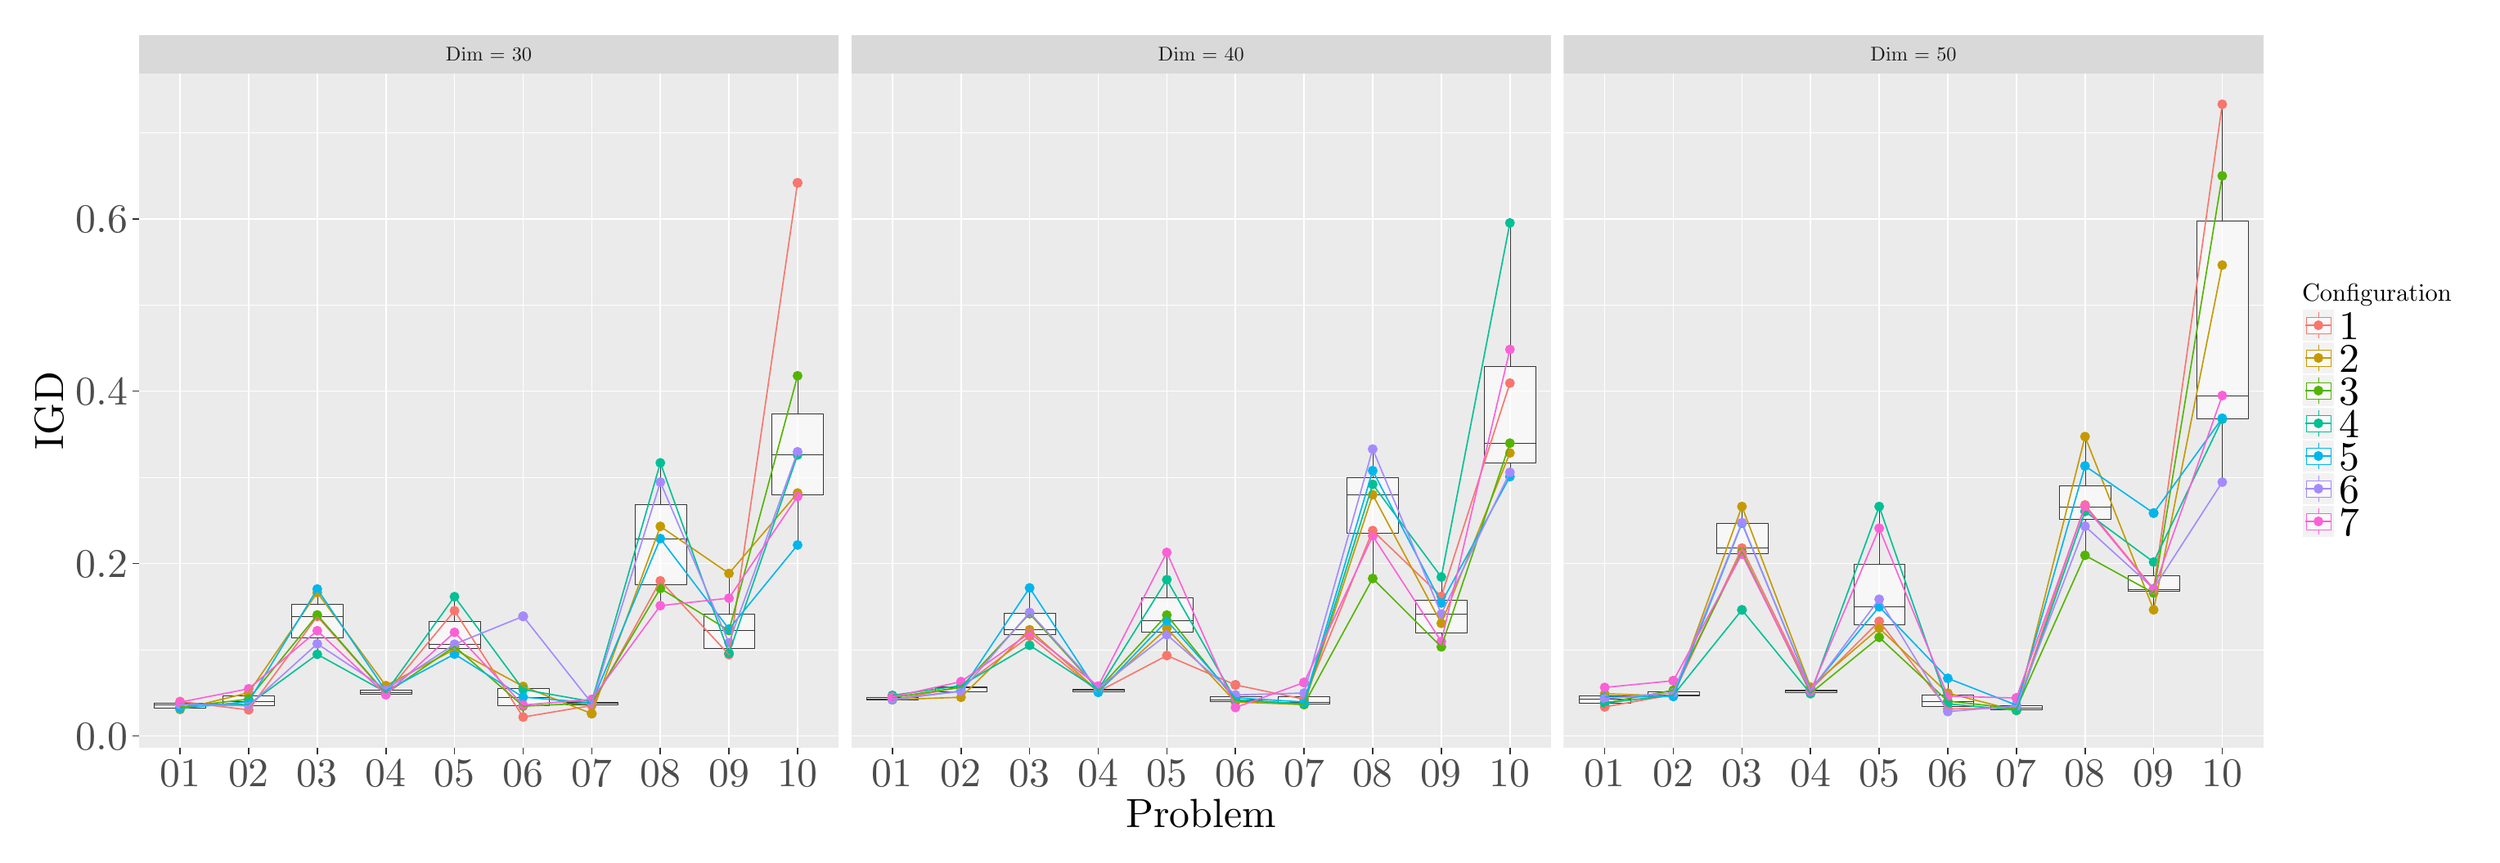
\begin{tikzpicture}[x=1pt,y=1pt]
\definecolor{fillColor}{RGB}{255,255,255}
\path[use as bounding box,fill=fillColor,fill opacity=0.00] (0,0) rectangle (1084.05,361.35);
\begin{scope}
\path[clip] (  0.00,  0.00) rectangle (1084.05,361.35);
\definecolor{drawColor}{RGB}{255,255,255}
\definecolor{fillColor}{RGB}{255,255,255}

\path[draw=drawColor,line width= 0.6pt,line join=round,line cap=round,fill=fillColor] (  0.00,  0.00) rectangle (1084.05,361.35);
\end{scope}
\begin{scope}
\path[clip] ( 51.34, 40.74) rectangle (360.49,338.79);
\definecolor{fillColor}{gray}{0.92}

\path[fill=fillColor] ( 51.34, 40.74) rectangle (360.49,338.79);
\definecolor{drawColor}{RGB}{255,255,255}

\path[draw=drawColor,line width= 0.3pt,line join=round] ( 51.34, 84.09) --
	(360.49, 84.09);

\path[draw=drawColor,line width= 0.3pt,line join=round] ( 51.34,160.30) --
	(360.49,160.30);

\path[draw=drawColor,line width= 0.3pt,line join=round] ( 51.34,236.50) --
	(360.49,236.50);

\path[draw=drawColor,line width= 0.3pt,line join=round] ( 51.34,312.71) --
	(360.49,312.71);

\path[draw=drawColor,line width= 0.6pt,line join=round] ( 51.34, 45.99) --
	(360.49, 45.99);

\path[draw=drawColor,line width= 0.6pt,line join=round] ( 51.34,122.20) --
	(360.49,122.20);

\path[draw=drawColor,line width= 0.6pt,line join=round] ( 51.34,198.40) --
	(360.49,198.40);

\path[draw=drawColor,line width= 0.6pt,line join=round] ( 51.34,274.61) --
	(360.49,274.61);

\path[draw=drawColor,line width= 0.6pt,line join=round] ( 69.53, 40.74) --
	( 69.53,338.79);

\path[draw=drawColor,line width= 0.6pt,line join=round] ( 99.83, 40.74) --
	( 99.83,338.79);

\path[draw=drawColor,line width= 0.6pt,line join=round] (130.14, 40.74) --
	(130.14,338.79);

\path[draw=drawColor,line width= 0.6pt,line join=round] (160.45, 40.74) --
	(160.45,338.79);

\path[draw=drawColor,line width= 0.6pt,line join=round] (190.76, 40.74) --
	(190.76,338.79);

\path[draw=drawColor,line width= 0.6pt,line join=round] (221.07, 40.74) --
	(221.07,338.79);

\path[draw=drawColor,line width= 0.6pt,line join=round] (251.38, 40.74) --
	(251.38,338.79);

\path[draw=drawColor,line width= 0.6pt,line join=round] (281.68, 40.74) --
	(281.68,338.79);

\path[draw=drawColor,line width= 0.6pt,line join=round] (311.99, 40.74) --
	(311.99,338.79);

\path[draw=drawColor,line width= 0.6pt,line join=round] (342.30, 40.74) --
	(342.30,338.79);
\definecolor{drawColor}{gray}{0.20}

\path[draw=drawColor,line width= 0.1pt,line join=round] ( 69.53, 60.50) -- ( 69.53, 61.16);

\path[draw=drawColor,line width= 0.1pt,line join=round] ( 69.53, 58.42) -- ( 69.53, 57.64);
\definecolor{fillColor}{RGB}{255,255,255}

\path[draw=drawColor,line width= 0.1pt,line join=round,line cap=round,fill=fillColor,fill opacity=0.60] ( 58.16, 60.50) --
	( 58.16, 58.42) --
	( 80.89, 58.42) --
	( 80.89, 60.50) --
	( 58.16, 60.50) --
	cycle;

\path[draw=drawColor,line width= 0.2pt,line join=round] ( 58.16, 59.87) -- ( 80.89, 59.87);

\path[draw=drawColor,line width= 0.1pt,line join=round] ( 99.83, 63.62) -- ( 99.83, 66.79);

\path[draw=drawColor,line width= 0.1pt,line join=round] ( 99.83, 59.55) -- ( 99.83, 57.46);

\path[draw=drawColor,line width= 0.1pt,line join=round,line cap=round,fill=fillColor,fill opacity=0.60] ( 88.47, 63.62) --
	( 88.47, 59.55) --
	(111.20, 59.55) --
	(111.20, 63.62) --
	( 88.47, 63.62) --
	cycle;

\path[draw=drawColor,line width= 0.2pt,line join=round] ( 88.47, 61.09) -- (111.20, 61.09);

\path[draw=drawColor,line width= 0.1pt,line join=round] (130.14,104.39) -- (130.14,110.91);

\path[draw=drawColor,line width= 0.1pt,line join=round] (130.14, 89.57) -- (130.14, 82.03);

\path[draw=drawColor,line width= 0.1pt,line join=round,line cap=round,fill=fillColor,fill opacity=0.60] (118.78,104.39) --
	(118.78, 89.57) --
	(141.51, 89.57) --
	(141.51,104.39) --
	(118.78,104.39) --
	cycle;

\path[draw=drawColor,line width= 0.2pt,line join=round] (118.78, 98.82) -- (141.51, 98.82);

\path[draw=drawColor,line width= 0.1pt,line join=round] (160.45, 66.18) -- (160.45, 68.17);

\path[draw=drawColor,line width= 0.1pt,line join=round] (160.45, 64.64) -- (160.45, 64.18);

\path[draw=drawColor,line width= 0.1pt,line join=round,line cap=round,fill=fillColor,fill opacity=0.60] (149.09, 66.18) --
	(149.09, 64.64) --
	(171.82, 64.64) --
	(171.82, 66.18) --
	(149.09, 66.18) --
	cycle;

\path[draw=drawColor,line width= 0.2pt,line join=round] (149.09, 65.27) -- (171.82, 65.27);

\path[draw=drawColor,line width= 0.1pt,line join=round] (190.76, 96.52) -- (190.76,107.51);

\path[draw=drawColor,line width= 0.1pt,line join=round] (190.76, 84.86) -- (190.76, 82.13);

\path[draw=drawColor,line width= 0.1pt,line join=round,line cap=round,fill=fillColor,fill opacity=0.60] (179.39, 96.52) --
	(179.39, 84.86) --
	(202.12, 84.86) --
	(202.12, 96.52) --
	(179.39, 96.52) --
	cycle;

\path[draw=drawColor,line width= 0.2pt,line join=round] (179.39, 86.51) -- (202.12, 86.51);
\definecolor{drawColor}{RGB}{51,51,51}
\definecolor{fillColor}{RGB}{51,51,51}

\path[draw=drawColor,draw opacity=0.60,line width= 0.4pt,line join=round,line cap=round,fill=fillColor,fill opacity=0.60] (221.07, 98.82) circle (  1.96);
\definecolor{drawColor}{gray}{0.20}

\path[draw=drawColor,line width= 0.1pt,line join=round] (221.07, 67.16) -- (221.07, 67.83);

\path[draw=drawColor,line width= 0.1pt,line join=round] (221.07, 59.37) -- (221.07, 54.29);
\definecolor{fillColor}{RGB}{255,255,255}

\path[draw=drawColor,line width= 0.1pt,line join=round,line cap=round,fill=fillColor,fill opacity=0.60] (209.70, 67.16) --
	(209.70, 59.37) --
	(232.43, 59.37) --
	(232.43, 67.16) --
	(209.70, 67.16) --
	cycle;

\path[draw=drawColor,line width= 0.2pt,line join=round] (209.70, 63.11) -- (232.43, 63.11);
\definecolor{drawColor}{RGB}{51,51,51}
\definecolor{fillColor}{RGB}{51,51,51}

\path[draw=drawColor,draw opacity=0.60,line width= 0.4pt,line join=round,line cap=round,fill=fillColor,fill opacity=0.60] (251.38, 55.80) circle (  1.96);
\definecolor{drawColor}{gray}{0.20}

\path[draw=drawColor,line width= 0.1pt,line join=round] (251.38, 60.86) -- (251.38, 62.11);

\path[draw=drawColor,line width= 0.1pt,line join=round] (251.38, 59.91) -- (251.38, 59.39);
\definecolor{fillColor}{RGB}{255,255,255}

\path[draw=drawColor,line width= 0.1pt,line join=round,line cap=round,fill=fillColor,fill opacity=0.60] (240.01, 60.86) --
	(240.01, 59.91) --
	(262.74, 59.91) --
	(262.74, 60.86) --
	(240.01, 60.86) --
	cycle;

\path[draw=drawColor,line width= 0.2pt,line join=round] (240.01, 60.46) -- (262.74, 60.46);

\path[draw=drawColor,line width= 0.1pt,line join=round] (281.68,148.39) -- (281.68,166.69);

\path[draw=drawColor,line width= 0.1pt,line join=round] (281.68,112.85) -- (281.68,103.55);

\path[draw=drawColor,line width= 0.1pt,line join=round,line cap=round,fill=fillColor,fill opacity=0.60] (270.32,148.39) --
	(270.32,112.85) --
	(293.05,112.85) --
	(293.05,148.39) --
	(270.32,148.39) --
	cycle;

\path[draw=drawColor,line width= 0.2pt,line join=round] (270.32,133.21) -- (293.05,133.21);

\path[draw=drawColor,line width= 0.1pt,line join=round] (311.99,100.04) -- (311.99,117.79);

\path[draw=drawColor,line width= 0.1pt,line join=round] (311.99, 84.82) -- (311.99, 81.92);

\path[draw=drawColor,line width= 0.1pt,line join=round,line cap=round,fill=fillColor,fill opacity=0.60] (300.63,100.04) --
	(300.63, 84.82) --
	(323.36, 84.82) --
	(323.36,100.04) --
	(300.63,100.04) --
	cycle;

\path[draw=drawColor,line width= 0.2pt,line join=round] (300.63, 92.56) -- (323.36, 92.56);
\definecolor{drawColor}{RGB}{51,51,51}
\definecolor{fillColor}{RGB}{51,51,51}

\path[draw=drawColor,draw opacity=0.60,line width= 0.4pt,line join=round,line cap=round,fill=fillColor,fill opacity=0.60] (342.30,290.51) circle (  1.96);
\definecolor{drawColor}{gray}{0.20}

\path[draw=drawColor,line width= 0.1pt,line join=round] (342.30,188.39) -- (342.30,205.18);

\path[draw=drawColor,line width= 0.1pt,line join=round] (342.30,152.58) -- (342.30,130.38);
\definecolor{fillColor}{RGB}{255,255,255}

\path[draw=drawColor,line width= 0.1pt,line join=round,line cap=round,fill=fillColor,fill opacity=0.60] (330.93,188.39) --
	(330.93,152.58) --
	(353.67,152.58) --
	(353.67,188.39) --
	(330.93,188.39) --
	cycle;

\path[draw=drawColor,line width= 0.2pt,line join=round] (330.93,170.21) -- (353.67,170.21);
\definecolor{drawColor}{RGB}{248,118,109}
\definecolor{fillColor}{RGB}{248,118,109}

\path[draw=drawColor,line width= 0.4pt,line join=round,line cap=round,fill=fillColor] ( 69.53, 61.16) circle (  1.96);

\path[draw=drawColor,line width= 0.4pt,line join=round,line cap=round,fill=fillColor] ( 99.83, 57.46) circle (  1.96);

\path[draw=drawColor,line width= 0.4pt,line join=round,line cap=round,fill=fillColor] (130.14, 98.82) circle (  1.96);

\path[draw=drawColor,line width= 0.4pt,line join=round,line cap=round,fill=fillColor] (160.45, 64.57) circle (  1.96);

\path[draw=drawColor,line width= 0.4pt,line join=round,line cap=round,fill=fillColor] (190.76,101.30) circle (  1.96);

\path[draw=drawColor,line width= 0.4pt,line join=round,line cap=round,fill=fillColor] (221.07, 54.29) circle (  1.96);

\path[draw=drawColor,line width= 0.4pt,line join=round,line cap=round,fill=fillColor] (251.38, 59.39) circle (  1.96);

\path[draw=drawColor,line width= 0.4pt,line join=round,line cap=round,fill=fillColor] (281.68,114.53) circle (  1.96);

\path[draw=drawColor,line width= 0.4pt,line join=round,line cap=round,fill=fillColor] (311.99, 81.92) circle (  1.96);

\path[draw=drawColor,line width= 0.4pt,line join=round,line cap=round,fill=fillColor] (342.30,290.51) circle (  1.96);
\definecolor{drawColor}{RGB}{196,154,0}
\definecolor{fillColor}{RGB}{196,154,0}

\path[draw=drawColor,line width= 0.4pt,line join=round,line cap=round,fill=fillColor] ( 69.53, 57.64) circle (  1.96);

\path[draw=drawColor,line width= 0.4pt,line join=round,line cap=round,fill=fillColor] ( 99.83, 65.04) circle (  1.96);

\path[draw=drawColor,line width= 0.4pt,line join=round,line cap=round,fill=fillColor] (130.14,109.34) circle (  1.96);

\path[draw=drawColor,line width= 0.4pt,line join=round,line cap=round,fill=fillColor] (160.45, 68.17) circle (  1.96);

\path[draw=drawColor,line width= 0.4pt,line join=round,line cap=round,fill=fillColor] (190.76, 84.21) circle (  1.96);

\path[draw=drawColor,line width= 0.4pt,line join=round,line cap=round,fill=fillColor] (221.07, 67.83) circle (  1.96);

\path[draw=drawColor,line width= 0.4pt,line join=round,line cap=round,fill=fillColor] (251.38, 55.80) circle (  1.96);

\path[draw=drawColor,line width= 0.4pt,line join=round,line cap=round,fill=fillColor] (281.68,138.61) circle (  1.96);

\path[draw=drawColor,line width= 0.4pt,line join=round,line cap=round,fill=fillColor] (311.99,117.79) circle (  1.96);

\path[draw=drawColor,line width= 0.4pt,line join=round,line cap=round,fill=fillColor] (342.30,153.35) circle (  1.96);
\definecolor{drawColor}{RGB}{83,180,0}
\definecolor{fillColor}{RGB}{83,180,0}

\path[draw=drawColor,line width= 0.4pt,line join=round,line cap=round,fill=fillColor] ( 69.53, 58.69) circle (  1.96);

\path[draw=drawColor,line width= 0.4pt,line join=round,line cap=round,fill=fillColor] ( 99.83, 62.21) circle (  1.96);

\path[draw=drawColor,line width= 0.4pt,line join=round,line cap=round,fill=fillColor] (130.14, 99.44) circle (  1.96);

\path[draw=drawColor,line width= 0.4pt,line join=round,line cap=round,fill=fillColor] (160.45, 64.70) circle (  1.96);

\path[draw=drawColor,line width= 0.4pt,line join=round,line cap=round,fill=fillColor] (190.76, 85.51) circle (  1.96);

\path[draw=drawColor,line width= 0.4pt,line join=round,line cap=round,fill=fillColor] (221.07, 59.13) circle (  1.96);

\path[draw=drawColor,line width= 0.4pt,line join=round,line cap=round,fill=fillColor] (251.38, 60.46) circle (  1.96);

\path[draw=drawColor,line width= 0.4pt,line join=round,line cap=round,fill=fillColor] (281.68,111.17) circle (  1.96);

\path[draw=drawColor,line width= 0.4pt,line join=round,line cap=round,fill=fillColor] (311.99, 92.56) circle (  1.96);

\path[draw=drawColor,line width= 0.4pt,line join=round,line cap=round,fill=fillColor] (342.30,205.18) circle (  1.96);
\definecolor{drawColor}{RGB}{0,192,148}
\definecolor{fillColor}{RGB}{0,192,148}

\path[draw=drawColor,line width= 0.4pt,line join=round,line cap=round,fill=fillColor] ( 69.53, 60.11) circle (  1.96);

\path[draw=drawColor,line width= 0.4pt,line join=round,line cap=round,fill=fillColor] ( 99.83, 59.81) circle (  1.96);

\path[draw=drawColor,line width= 0.4pt,line join=round,line cap=round,fill=fillColor] (130.14, 82.03) circle (  1.96);

\path[draw=drawColor,line width= 0.4pt,line join=round,line cap=round,fill=fillColor] (160.45, 65.27) circle (  1.96);

\path[draw=drawColor,line width= 0.4pt,line join=round,line cap=round,fill=fillColor] (190.76,107.51) circle (  1.96);

\path[draw=drawColor,line width= 0.4pt,line join=round,line cap=round,fill=fillColor] (221.07, 66.49) circle (  1.96);

\path[draw=drawColor,line width= 0.4pt,line join=round,line cap=round,fill=fillColor] (251.38, 61.14) circle (  1.96);

\path[draw=drawColor,line width= 0.4pt,line join=round,line cap=round,fill=fillColor] (281.68,166.69) circle (  1.96);

\path[draw=drawColor,line width= 0.4pt,line join=round,line cap=round,fill=fillColor] (311.99, 82.52) circle (  1.96);

\path[draw=drawColor,line width= 0.4pt,line join=round,line cap=round,fill=fillColor] (342.30,170.21) circle (  1.96);
\definecolor{drawColor}{RGB}{0,182,235}
\definecolor{fillColor}{RGB}{0,182,235}

\path[draw=drawColor,line width= 0.4pt,line join=round,line cap=round,fill=fillColor] ( 69.53, 58.14) circle (  1.96);

\path[draw=drawColor,line width= 0.4pt,line join=round,line cap=round,fill=fillColor] ( 99.83, 61.09) circle (  1.96);

\path[draw=drawColor,line width= 0.4pt,line join=round,line cap=round,fill=fillColor] (130.14,110.91) circle (  1.96);

\path[draw=drawColor,line width= 0.4pt,line join=round,line cap=round,fill=fillColor] (160.45, 65.77) circle (  1.96);

\path[draw=drawColor,line width= 0.4pt,line join=round,line cap=round,fill=fillColor] (190.76, 82.13) circle (  1.96);

\path[draw=drawColor,line width= 0.4pt,line join=round,line cap=round,fill=fillColor] (221.07, 63.11) circle (  1.96);

\path[draw=drawColor,line width= 0.4pt,line join=round,line cap=round,fill=fillColor] (251.38, 60.59) circle (  1.96);

\path[draw=drawColor,line width= 0.4pt,line join=round,line cap=round,fill=fillColor] (281.68,133.21) circle (  1.96);

\path[draw=drawColor,line width= 0.4pt,line join=round,line cap=round,fill=fillColor] (311.99, 93.21) circle (  1.96);

\path[draw=drawColor,line width= 0.4pt,line join=round,line cap=round,fill=fillColor] (342.30,130.38) circle (  1.96);
\definecolor{drawColor}{RGB}{165,138,255}
\definecolor{fillColor}{RGB}{165,138,255}

\path[draw=drawColor,line width= 0.4pt,line join=round,line cap=round,fill=fillColor] ( 69.53, 59.87) circle (  1.96);

\path[draw=drawColor,line width= 0.4pt,line join=round,line cap=round,fill=fillColor] ( 99.83, 59.28) circle (  1.96);

\path[draw=drawColor,line width= 0.4pt,line join=round,line cap=round,fill=fillColor] (130.14, 86.68) circle (  1.96);

\path[draw=drawColor,line width= 0.4pt,line join=round,line cap=round,fill=fillColor] (160.45, 66.59) circle (  1.96);

\path[draw=drawColor,line width= 0.4pt,line join=round,line cap=round,fill=fillColor] (190.76, 86.51) circle (  1.96);

\path[draw=drawColor,line width= 0.4pt,line join=round,line cap=round,fill=fillColor] (221.07, 98.82) circle (  1.96);

\path[draw=drawColor,line width= 0.4pt,line join=round,line cap=round,fill=fillColor] (251.38, 60.43) circle (  1.96);

\path[draw=drawColor,line width= 0.4pt,line join=round,line cap=round,fill=fillColor] (281.68,158.17) circle (  1.96);

\path[draw=drawColor,line width= 0.4pt,line join=round,line cap=round,fill=fillColor] (311.99, 87.11) circle (  1.96);

\path[draw=drawColor,line width= 0.4pt,line join=round,line cap=round,fill=fillColor] (342.30,171.59) circle (  1.96);
\definecolor{drawColor}{RGB}{251,97,215}
\definecolor{fillColor}{RGB}{251,97,215}

\path[draw=drawColor,line width= 0.4pt,line join=round,line cap=round,fill=fillColor] ( 69.53, 60.88) circle (  1.96);

\path[draw=drawColor,line width= 0.4pt,line join=round,line cap=round,fill=fillColor] ( 99.83, 66.79) circle (  1.96);

\path[draw=drawColor,line width= 0.4pt,line join=round,line cap=round,fill=fillColor] (130.14, 92.46) circle (  1.96);

\path[draw=drawColor,line width= 0.4pt,line join=round,line cap=round,fill=fillColor] (160.45, 64.18) circle (  1.96);

\path[draw=drawColor,line width= 0.4pt,line join=round,line cap=round,fill=fillColor] (190.76, 91.75) circle (  1.96);

\path[draw=drawColor,line width= 0.4pt,line join=round,line cap=round,fill=fillColor] (221.07, 59.61) circle (  1.96);

\path[draw=drawColor,line width= 0.4pt,line join=round,line cap=round,fill=fillColor] (251.38, 62.11) circle (  1.96);

\path[draw=drawColor,line width= 0.4pt,line join=round,line cap=round,fill=fillColor] (281.68,103.55) circle (  1.96);

\path[draw=drawColor,line width= 0.4pt,line join=round,line cap=round,fill=fillColor] (311.99,106.87) circle (  1.96);

\path[draw=drawColor,line width= 0.4pt,line join=round,line cap=round,fill=fillColor] (342.30,151.80) circle (  1.96);
\definecolor{drawColor}{RGB}{248,118,109}

\path[draw=drawColor,line width= 0.6pt,line join=round] ( 69.53, 61.16) --
	( 99.83, 57.46) --
	(130.14, 98.82) --
	(160.45, 64.57) --
	(190.76,101.30) --
	(221.07, 54.29) --
	(251.38, 59.39) --
	(281.68,114.53) --
	(311.99, 81.92) --
	(342.30,290.51);
\definecolor{drawColor}{RGB}{196,154,0}

\path[draw=drawColor,line width= 0.6pt,line join=round] ( 69.53, 57.64) --
	( 99.83, 65.04) --
	(130.14,109.34) --
	(160.45, 68.17) --
	(190.76, 84.21) --
	(221.07, 67.83) --
	(251.38, 55.80) --
	(281.68,138.61) --
	(311.99,117.79) --
	(342.30,153.35);
\definecolor{drawColor}{RGB}{83,180,0}

\path[draw=drawColor,line width= 0.6pt,line join=round] ( 69.53, 58.69) --
	( 99.83, 62.21) --
	(130.14, 99.44) --
	(160.45, 64.70) --
	(190.76, 85.51) --
	(221.07, 59.13) --
	(251.38, 60.46) --
	(281.68,111.17) --
	(311.99, 92.56) --
	(342.30,205.18);
\definecolor{drawColor}{RGB}{0,192,148}

\path[draw=drawColor,line width= 0.6pt,line join=round] ( 69.53, 60.11) --
	( 99.83, 59.81) --
	(130.14, 82.03) --
	(160.45, 65.27) --
	(190.76,107.51) --
	(221.07, 66.49) --
	(251.38, 61.14) --
	(281.68,166.69) --
	(311.99, 82.52) --
	(342.30,170.21);
\definecolor{drawColor}{RGB}{0,182,235}

\path[draw=drawColor,line width= 0.6pt,line join=round] ( 69.53, 58.14) --
	( 99.83, 61.09) --
	(130.14,110.91) --
	(160.45, 65.77) --
	(190.76, 82.13) --
	(221.07, 63.11) --
	(251.38, 60.59) --
	(281.68,133.21) --
	(311.99, 93.21) --
	(342.30,130.38);
\definecolor{drawColor}{RGB}{165,138,255}

\path[draw=drawColor,line width= 0.6pt,line join=round] ( 69.53, 59.87) --
	( 99.83, 59.28) --
	(130.14, 86.68) --
	(160.45, 66.59) --
	(190.76, 86.51) --
	(221.07, 98.82) --
	(251.38, 60.43) --
	(281.68,158.17) --
	(311.99, 87.11) --
	(342.30,171.59);
\definecolor{drawColor}{RGB}{251,97,215}

\path[draw=drawColor,line width= 0.6pt,line join=round] ( 69.53, 60.88) --
	( 99.83, 66.79) --
	(130.14, 92.46) --
	(160.45, 64.18) --
	(190.76, 91.75) --
	(221.07, 59.61) --
	(251.38, 62.11) --
	(281.68,103.55) --
	(311.99,106.87) --
	(342.30,151.80);
\end{scope}
\begin{scope}
\path[clip] (365.99, 40.74) rectangle (675.13,338.79);
\definecolor{fillColor}{gray}{0.92}

\path[fill=fillColor] (365.99, 40.74) rectangle (675.13,338.79);
\definecolor{drawColor}{RGB}{255,255,255}

\path[draw=drawColor,line width= 0.3pt,line join=round] (365.99, 84.09) --
	(675.13, 84.09);

\path[draw=drawColor,line width= 0.3pt,line join=round] (365.99,160.30) --
	(675.13,160.30);

\path[draw=drawColor,line width= 0.3pt,line join=round] (365.99,236.50) --
	(675.13,236.50);

\path[draw=drawColor,line width= 0.3pt,line join=round] (365.99,312.71) --
	(675.13,312.71);

\path[draw=drawColor,line width= 0.6pt,line join=round] (365.99, 45.99) --
	(675.13, 45.99);

\path[draw=drawColor,line width= 0.6pt,line join=round] (365.99,122.20) --
	(675.13,122.20);

\path[draw=drawColor,line width= 0.6pt,line join=round] (365.99,198.40) --
	(675.13,198.40);

\path[draw=drawColor,line width= 0.6pt,line join=round] (365.99,274.61) --
	(675.13,274.61);

\path[draw=drawColor,line width= 0.6pt,line join=round] (384.17, 40.74) --
	(384.17,338.79);

\path[draw=drawColor,line width= 0.6pt,line join=round] (414.48, 40.74) --
	(414.48,338.79);

\path[draw=drawColor,line width= 0.6pt,line join=round] (444.79, 40.74) --
	(444.79,338.79);

\path[draw=drawColor,line width= 0.6pt,line join=round] (475.09, 40.74) --
	(475.09,338.79);

\path[draw=drawColor,line width= 0.6pt,line join=round] (505.40, 40.74) --
	(505.40,338.79);

\path[draw=drawColor,line width= 0.6pt,line join=round] (535.71, 40.74) --
	(535.71,338.79);

\path[draw=drawColor,line width= 0.6pt,line join=round] (566.02, 40.74) --
	(566.02,338.79);

\path[draw=drawColor,line width= 0.6pt,line join=round] (596.33, 40.74) --
	(596.33,338.79);

\path[draw=drawColor,line width= 0.6pt,line join=round] (626.64, 40.74) --
	(626.64,338.79);

\path[draw=drawColor,line width= 0.6pt,line join=round] (656.94, 40.74) --
	(656.94,338.79);
\definecolor{drawColor}{gray}{0.20}

\path[draw=drawColor,line width= 0.1pt,line join=round] (384.17, 63.08) -- (384.17, 63.91);

\path[draw=drawColor,line width= 0.1pt,line join=round] (384.17, 62.01) -- (384.17, 61.94);
\definecolor{fillColor}{RGB}{255,255,255}

\path[draw=drawColor,line width= 0.1pt,line join=round,line cap=round,fill=fillColor,fill opacity=0.60] (372.80, 63.08) --
	(372.80, 62.01) --
	(395.54, 62.01) --
	(395.54, 63.08) --
	(372.80, 63.08) --
	cycle;

\path[draw=drawColor,line width= 0.2pt,line join=round] (372.80, 62.17) -- (395.54, 62.17);

\path[draw=drawColor,line width= 0.1pt,line join=round] (414.48, 67.85) -- (414.48, 69.94);

\path[draw=drawColor,line width= 0.1pt,line join=round] (414.48, 65.75) -- (414.48, 63.04);

\path[draw=drawColor,line width= 0.1pt,line join=round,line cap=round,fill=fillColor,fill opacity=0.60] (403.11, 67.85) --
	(403.11, 65.75) --
	(425.84, 65.75) --
	(425.84, 67.85) --
	(403.11, 67.85) --
	cycle;

\path[draw=drawColor,line width= 0.2pt,line join=round] (403.11, 67.47) -- (425.84, 67.47);

\path[draw=drawColor,line width= 0.1pt,line join=round] (444.79,100.27) -- (444.79,111.40);

\path[draw=drawColor,line width= 0.1pt,line join=round] (444.79, 90.78) -- (444.79, 86.02);

\path[draw=drawColor,line width= 0.1pt,line join=round,line cap=round,fill=fillColor,fill opacity=0.60] (433.42,100.27) --
	(433.42, 90.78) --
	(456.15, 90.78) --
	(456.15,100.27) --
	(433.42,100.27) --
	cycle;

\path[draw=drawColor,line width= 0.2pt,line join=round] (433.42, 92.88) -- (456.15, 92.88);

\path[draw=drawColor,line width= 0.1pt,line join=round] (475.09, 66.80) -- (475.09, 67.98);

\path[draw=drawColor,line width= 0.1pt,line join=round] (475.09, 65.62) -- (475.09, 65.20);

\path[draw=drawColor,line width= 0.1pt,line join=round,line cap=round,fill=fillColor,fill opacity=0.60] (463.73, 66.80) --
	(463.73, 65.62) --
	(486.46, 65.62) --
	(486.46, 66.80) --
	(463.73, 66.80) --
	cycle;

\path[draw=drawColor,line width= 0.2pt,line join=round] (463.73, 66.32) -- (486.46, 66.32);

\path[draw=drawColor,line width= 0.1pt,line join=round] (505.40,107.21) -- (505.40,127.08);

\path[draw=drawColor,line width= 0.1pt,line join=round] (505.40, 92.10) -- (505.40, 81.49);

\path[draw=drawColor,line width= 0.1pt,line join=round,line cap=round,fill=fillColor,fill opacity=0.60] (494.04,107.21) --
	(494.04, 92.10) --
	(516.77, 92.10) --
	(516.77,107.21) --
	(494.04,107.21) --
	cycle;

\path[draw=drawColor,line width= 0.2pt,line join=round] (494.04, 96.90) -- (516.77, 96.90);
\definecolor{drawColor}{RGB}{51,51,51}
\definecolor{fillColor}{RGB}{51,51,51}

\path[draw=drawColor,draw opacity=0.60,line width= 0.4pt,line join=round,line cap=round,fill=fillColor,fill opacity=0.60] (535.71, 68.51) circle (  1.96);
\definecolor{drawColor}{gray}{0.20}

\path[draw=drawColor,line width= 0.1pt,line join=round] (535.71, 63.44) -- (535.71, 64.07);

\path[draw=drawColor,line width= 0.1pt,line join=round] (535.71, 61.38) -- (535.71, 58.49);
\definecolor{fillColor}{RGB}{255,255,255}

\path[draw=drawColor,line width= 0.1pt,line join=round,line cap=round,fill=fillColor,fill opacity=0.60] (524.35, 63.44) --
	(524.35, 61.38) --
	(547.08, 61.38) --
	(547.08, 63.44) --
	(524.35, 63.44) --
	cycle;

\path[draw=drawColor,line width= 0.2pt,line join=round] (524.35, 61.91) -- (547.08, 61.91);
\definecolor{drawColor}{RGB}{51,51,51}
\definecolor{fillColor}{RGB}{51,51,51}

\path[draw=drawColor,draw opacity=0.60,line width= 0.4pt,line join=round,line cap=round,fill=fillColor,fill opacity=0.60] (566.02, 69.56) circle (  1.96);
\definecolor{drawColor}{gray}{0.20}

\path[draw=drawColor,line width= 0.1pt,line join=round] (566.02, 63.53) -- (566.02, 64.92);

\path[draw=drawColor,line width= 0.1pt,line join=round] (566.02, 60.03) -- (566.02, 59.80);
\definecolor{fillColor}{RGB}{255,255,255}

\path[draw=drawColor,line width= 0.1pt,line join=round,line cap=round,fill=fillColor,fill opacity=0.60] (554.65, 63.53) --
	(554.65, 60.03) --
	(577.39, 60.03) --
	(577.39, 63.53) --
	(554.65, 63.53) --
	cycle;

\path[draw=drawColor,line width= 0.2pt,line join=round] (554.65, 60.96) -- (577.39, 60.96);

\path[draw=drawColor,line width= 0.1pt,line join=round] (596.33,160.23) -- (596.33,172.78);

\path[draw=drawColor,line width= 0.1pt,line join=round] (596.33,135.56) -- (596.33,115.57);

\path[draw=drawColor,line width= 0.1pt,line join=round,line cap=round,fill=fillColor,fill opacity=0.60] (584.96,160.23) --
	(584.96,135.56) --
	(607.69,135.56) --
	(607.69,160.23) --
	(584.96,160.23) --
	cycle;

\path[draw=drawColor,line width= 0.2pt,line join=round] (584.96,152.61) -- (607.69,152.61);

\path[draw=drawColor,line width= 0.1pt,line join=round] (626.64,106.17) -- (626.64,116.21);

\path[draw=drawColor,line width= 0.1pt,line join=round] (626.64, 91.72) -- (626.64, 85.33);

\path[draw=drawColor,line width= 0.1pt,line join=round,line cap=round,fill=fillColor,fill opacity=0.60] (615.27,106.17) --
	(615.27, 91.72) --
	(638.00, 91.72) --
	(638.00,106.17) --
	(615.27,106.17) --
	cycle;

\path[draw=drawColor,line width= 0.2pt,line join=round] (615.27, 99.86) -- (638.00, 99.86);

\path[draw=drawColor,line width= 0.1pt,line join=round] (656.94,209.40) -- (656.94,272.77);

\path[draw=drawColor,line width= 0.1pt,line join=round] (656.94,166.78) -- (656.94,160.58);

\path[draw=drawColor,line width= 0.1pt,line join=round,line cap=round,fill=fillColor,fill opacity=0.60] (645.58,209.40) --
	(645.58,166.78) --
	(668.31,166.78) --
	(668.31,209.40) --
	(645.58,209.40) --
	cycle;

\path[draw=drawColor,line width= 0.2pt,line join=round] (645.58,175.40) -- (668.31,175.40);
\definecolor{drawColor}{RGB}{248,118,109}
\definecolor{fillColor}{RGB}{248,118,109}

\path[draw=drawColor,line width= 0.4pt,line join=round,line cap=round,fill=fillColor] (384.17, 61.94) circle (  1.96);

\path[draw=drawColor,line width= 0.4pt,line join=round,line cap=round,fill=fillColor] (414.48, 67.50) circle (  1.96);

\path[draw=drawColor,line width= 0.4pt,line join=round,line cap=round,fill=fillColor] (444.79, 90.09) circle (  1.96);

\path[draw=drawColor,line width= 0.4pt,line join=round,line cap=round,fill=fillColor] (475.09, 65.52) circle (  1.96);

\path[draw=drawColor,line width= 0.4pt,line join=round,line cap=round,fill=fillColor] (505.40, 81.49) circle (  1.96);

\path[draw=drawColor,line width= 0.4pt,line join=round,line cap=round,fill=fillColor] (535.71, 68.51) circle (  1.96);

\path[draw=drawColor,line width= 0.4pt,line join=round,line cap=round,fill=fillColor] (566.02, 62.15) circle (  1.96);

\path[draw=drawColor,line width= 0.4pt,line join=round,line cap=round,fill=fillColor] (596.33,136.75) circle (  1.96);

\path[draw=drawColor,line width= 0.4pt,line join=round,line cap=round,fill=fillColor] (626.64,107.62) circle (  1.96);

\path[draw=drawColor,line width= 0.4pt,line join=round,line cap=round,fill=fillColor] (656.94,201.95) circle (  1.96);
\definecolor{drawColor}{RGB}{196,154,0}
\definecolor{fillColor}{RGB}{196,154,0}

\path[draw=drawColor,line width= 0.4pt,line join=round,line cap=round,fill=fillColor] (384.17, 62.02) circle (  1.96);

\path[draw=drawColor,line width= 0.4pt,line join=round,line cap=round,fill=fillColor] (414.48, 63.04) circle (  1.96);

\path[draw=drawColor,line width= 0.4pt,line join=round,line cap=round,fill=fillColor] (444.79, 92.88) circle (  1.96);

\path[draw=drawColor,line width= 0.4pt,line join=round,line cap=round,fill=fillColor] (475.09, 65.71) circle (  1.96);

\path[draw=drawColor,line width= 0.4pt,line join=round,line cap=round,fill=fillColor] (505.40, 93.47) circle (  1.96);

\path[draw=drawColor,line width= 0.4pt,line join=round,line cap=round,fill=fillColor] (535.71, 60.98) circle (  1.96);

\path[draw=drawColor,line width= 0.4pt,line join=round,line cap=round,fill=fillColor] (566.02, 59.80) circle (  1.96);

\path[draw=drawColor,line width= 0.4pt,line join=round,line cap=round,fill=fillColor] (596.33,152.61) circle (  1.96);

\path[draw=drawColor,line width= 0.4pt,line join=round,line cap=round,fill=fillColor] (626.64, 95.74) circle (  1.96);

\path[draw=drawColor,line width= 0.4pt,line join=round,line cap=round,fill=fillColor] (656.94,171.07) circle (  1.96);
\definecolor{drawColor}{RGB}{83,180,0}
\definecolor{fillColor}{RGB}{83,180,0}

\path[draw=drawColor,line width= 0.4pt,line join=round,line cap=round,fill=fillColor] (384.17, 62.95) circle (  1.96);

\path[draw=drawColor,line width= 0.4pt,line join=round,line cap=round,fill=fillColor] (414.48, 67.47) circle (  1.96);

\path[draw=drawColor,line width= 0.4pt,line join=round,line cap=round,fill=fillColor] (444.79,100.02) circle (  1.96);

\path[draw=drawColor,line width= 0.4pt,line join=round,line cap=round,fill=fillColor] (475.09, 66.51) circle (  1.96);

\path[draw=drawColor,line width= 0.4pt,line join=round,line cap=round,fill=fillColor] (505.40, 99.39) circle (  1.96);

\path[draw=drawColor,line width= 0.4pt,line join=round,line cap=round,fill=fillColor] (535.71, 61.78) circle (  1.96);

\path[draw=drawColor,line width= 0.4pt,line join=round,line cap=round,fill=fillColor] (566.02, 59.88) circle (  1.96);

\path[draw=drawColor,line width= 0.4pt,line join=round,line cap=round,fill=fillColor] (596.33,115.57) circle (  1.96);

\path[draw=drawColor,line width= 0.4pt,line join=round,line cap=round,fill=fillColor] (626.64, 85.33) circle (  1.96);

\path[draw=drawColor,line width= 0.4pt,line join=round,line cap=round,fill=fillColor] (656.94,175.40) circle (  1.96);
\definecolor{drawColor}{RGB}{0,192,148}
\definecolor{fillColor}{RGB}{0,192,148}

\path[draw=drawColor,line width= 0.4pt,line join=round,line cap=round,fill=fillColor] (384.17, 63.91) circle (  1.96);

\path[draw=drawColor,line width= 0.4pt,line join=round,line cap=round,fill=fillColor] (414.48, 68.20) circle (  1.96);

\path[draw=drawColor,line width= 0.4pt,line join=round,line cap=round,fill=fillColor] (444.79, 86.02) circle (  1.96);

\path[draw=drawColor,line width= 0.4pt,line join=round,line cap=round,fill=fillColor] (475.09, 66.32) circle (  1.96);

\path[draw=drawColor,line width= 0.4pt,line join=round,line cap=round,fill=fillColor] (505.40,115.04) circle (  1.96);

\path[draw=drawColor,line width= 0.4pt,line join=round,line cap=round,fill=fillColor] (535.71, 61.91) circle (  1.96);

\path[draw=drawColor,line width= 0.4pt,line join=round,line cap=round,fill=fillColor] (566.02, 60.19) circle (  1.96);

\path[draw=drawColor,line width= 0.4pt,line join=round,line cap=round,fill=fillColor] (596.33,157.19) circle (  1.96);

\path[draw=drawColor,line width= 0.4pt,line join=round,line cap=round,fill=fillColor] (626.64,116.21) circle (  1.96);

\path[draw=drawColor,line width= 0.4pt,line join=round,line cap=round,fill=fillColor] (656.94,272.77) circle (  1.96);
\definecolor{drawColor}{RGB}{0,182,235}
\definecolor{fillColor}{RGB}{0,182,235}

\path[draw=drawColor,line width= 0.4pt,line join=round,line cap=round,fill=fillColor] (384.17, 62.01) circle (  1.96);

\path[draw=drawColor,line width= 0.4pt,line join=round,line cap=round,fill=fillColor] (414.48, 65.85) circle (  1.96);

\path[draw=drawColor,line width= 0.4pt,line join=round,line cap=round,fill=fillColor] (444.79,111.40) circle (  1.96);

\path[draw=drawColor,line width= 0.4pt,line join=round,line cap=round,fill=fillColor] (475.09, 65.20) circle (  1.96);

\path[draw=drawColor,line width= 0.4pt,line join=round,line cap=round,fill=fillColor] (505.40, 96.90) circle (  1.96);

\path[draw=drawColor,line width= 0.4pt,line join=round,line cap=round,fill=fillColor] (535.71, 62.80) circle (  1.96);

\path[draw=drawColor,line width= 0.4pt,line join=round,line cap=round,fill=fillColor] (566.02, 60.96) circle (  1.96);

\path[draw=drawColor,line width= 0.4pt,line join=round,line cap=round,fill=fillColor] (596.33,163.26) circle (  1.96);

\path[draw=drawColor,line width= 0.4pt,line join=round,line cap=round,fill=fillColor] (626.64,104.73) circle (  1.96);

\path[draw=drawColor,line width= 0.4pt,line join=round,line cap=round,fill=fillColor] (656.94,160.58) circle (  1.96);
\definecolor{drawColor}{RGB}{165,138,255}
\definecolor{fillColor}{RGB}{165,138,255}

\path[draw=drawColor,line width= 0.4pt,line join=round,line cap=round,fill=fillColor] (384.17, 62.17) circle (  1.96);

\path[draw=drawColor,line width= 0.4pt,line join=round,line cap=round,fill=fillColor] (414.48, 65.65) circle (  1.96);

\path[draw=drawColor,line width= 0.4pt,line join=round,line cap=round,fill=fillColor] (444.79,100.52) circle (  1.96);

\path[draw=drawColor,line width= 0.4pt,line join=round,line cap=round,fill=fillColor] (475.09, 67.09) circle (  1.96);

\path[draw=drawColor,line width= 0.4pt,line join=round,line cap=round,fill=fillColor] (505.40, 90.72) circle (  1.96);

\path[draw=drawColor,line width= 0.4pt,line join=round,line cap=round,fill=fillColor] (535.71, 64.07) circle (  1.96);

\path[draw=drawColor,line width= 0.4pt,line join=round,line cap=round,fill=fillColor] (566.02, 64.92) circle (  1.96);

\path[draw=drawColor,line width= 0.4pt,line join=round,line cap=round,fill=fillColor] (596.33,172.78) circle (  1.96);

\path[draw=drawColor,line width= 0.4pt,line join=round,line cap=round,fill=fillColor] (626.64, 99.86) circle (  1.96);

\path[draw=drawColor,line width= 0.4pt,line join=round,line cap=round,fill=fillColor] (656.94,162.49) circle (  1.96);
\definecolor{drawColor}{RGB}{251,97,215}
\definecolor{fillColor}{RGB}{251,97,215}

\path[draw=drawColor,line width= 0.4pt,line join=round,line cap=round,fill=fillColor] (384.17, 63.21) circle (  1.96);

\path[draw=drawColor,line width= 0.4pt,line join=round,line cap=round,fill=fillColor] (414.48, 69.94) circle (  1.96);

\path[draw=drawColor,line width= 0.4pt,line join=round,line cap=round,fill=fillColor] (444.79, 91.47) circle (  1.96);

\path[draw=drawColor,line width= 0.4pt,line join=round,line cap=round,fill=fillColor] (475.09, 67.98) circle (  1.96);

\path[draw=drawColor,line width= 0.4pt,line join=round,line cap=round,fill=fillColor] (505.40,127.08) circle (  1.96);

\path[draw=drawColor,line width= 0.4pt,line join=round,line cap=round,fill=fillColor] (535.71, 58.49) circle (  1.96);

\path[draw=drawColor,line width= 0.4pt,line join=round,line cap=round,fill=fillColor] (566.02, 69.56) circle (  1.96);

\path[draw=drawColor,line width= 0.4pt,line join=round,line cap=round,fill=fillColor] (596.33,134.37) circle (  1.96);

\path[draw=drawColor,line width= 0.4pt,line join=round,line cap=round,fill=fillColor] (626.64, 87.70) circle (  1.96);

\path[draw=drawColor,line width= 0.4pt,line join=round,line cap=round,fill=fillColor] (656.94,216.84) circle (  1.96);
\definecolor{drawColor}{RGB}{248,118,109}

\path[draw=drawColor,line width= 0.6pt,line join=round] (384.17, 61.94) --
	(414.48, 67.50) --
	(444.79, 90.09) --
	(475.09, 65.52) --
	(505.40, 81.49) --
	(535.71, 68.51) --
	(566.02, 62.15) --
	(596.33,136.75) --
	(626.64,107.62) --
	(656.94,201.95);
\definecolor{drawColor}{RGB}{196,154,0}

\path[draw=drawColor,line width= 0.6pt,line join=round] (384.17, 62.02) --
	(414.48, 63.04) --
	(444.79, 92.88) --
	(475.09, 65.71) --
	(505.40, 93.47) --
	(535.71, 60.98) --
	(566.02, 59.80) --
	(596.33,152.61) --
	(626.64, 95.74) --
	(656.94,171.07);
\definecolor{drawColor}{RGB}{83,180,0}

\path[draw=drawColor,line width= 0.6pt,line join=round] (384.17, 62.95) --
	(414.48, 67.47) --
	(444.79,100.02) --
	(475.09, 66.51) --
	(505.40, 99.39) --
	(535.71, 61.78) --
	(566.02, 59.88) --
	(596.33,115.57) --
	(626.64, 85.33) --
	(656.94,175.40);
\definecolor{drawColor}{RGB}{0,192,148}

\path[draw=drawColor,line width= 0.6pt,line join=round] (384.17, 63.91) --
	(414.48, 68.20) --
	(444.79, 86.02) --
	(475.09, 66.32) --
	(505.40,115.04) --
	(535.71, 61.91) --
	(566.02, 60.19) --
	(596.33,157.19) --
	(626.64,116.21) --
	(656.94,272.77);
\definecolor{drawColor}{RGB}{0,182,235}

\path[draw=drawColor,line width= 0.6pt,line join=round] (384.17, 62.01) --
	(414.48, 65.85) --
	(444.79,111.40) --
	(475.09, 65.20) --
	(505.40, 96.90) --
	(535.71, 62.80) --
	(566.02, 60.96) --
	(596.33,163.26) --
	(626.64,104.73) --
	(656.94,160.58);
\definecolor{drawColor}{RGB}{165,138,255}

\path[draw=drawColor,line width= 0.6pt,line join=round] (384.17, 62.17) --
	(414.48, 65.65) --
	(444.79,100.52) --
	(475.09, 67.09) --
	(505.40, 90.72) --
	(535.71, 64.07) --
	(566.02, 64.92) --
	(596.33,172.78) --
	(626.64, 99.86) --
	(656.94,162.49);
\definecolor{drawColor}{RGB}{251,97,215}

\path[draw=drawColor,line width= 0.6pt,line join=round] (384.17, 63.21) --
	(414.48, 69.94) --
	(444.79, 91.47) --
	(475.09, 67.98) --
	(505.40,127.08) --
	(535.71, 58.49) --
	(566.02, 69.56) --
	(596.33,134.37) --
	(626.64, 87.70) --
	(656.94,216.84);
\end{scope}
\begin{scope}
\path[clip] (680.63, 40.74) rectangle (989.77,338.79);
\definecolor{fillColor}{gray}{0.92}

\path[fill=fillColor] (680.63, 40.74) rectangle (989.77,338.79);
\definecolor{drawColor}{RGB}{255,255,255}

\path[draw=drawColor,line width= 0.3pt,line join=round] (680.63, 84.09) --
	(989.77, 84.09);

\path[draw=drawColor,line width= 0.3pt,line join=round] (680.63,160.30) --
	(989.77,160.30);

\path[draw=drawColor,line width= 0.3pt,line join=round] (680.63,236.50) --
	(989.77,236.50);

\path[draw=drawColor,line width= 0.3pt,line join=round] (680.63,312.71) --
	(989.77,312.71);

\path[draw=drawColor,line width= 0.6pt,line join=round] (680.63, 45.99) --
	(989.77, 45.99);

\path[draw=drawColor,line width= 0.6pt,line join=round] (680.63,122.20) --
	(989.77,122.20);

\path[draw=drawColor,line width= 0.6pt,line join=round] (680.63,198.40) --
	(989.77,198.40);

\path[draw=drawColor,line width= 0.6pt,line join=round] (680.63,274.61) --
	(989.77,274.61);

\path[draw=drawColor,line width= 0.6pt,line join=round] (698.81, 40.74) --
	(698.81,338.79);

\path[draw=drawColor,line width= 0.6pt,line join=round] (729.12, 40.74) --
	(729.12,338.79);

\path[draw=drawColor,line width= 0.6pt,line join=round] (759.43, 40.74) --
	(759.43,338.79);

\path[draw=drawColor,line width= 0.6pt,line join=round] (789.74, 40.74) --
	(789.74,338.79);

\path[draw=drawColor,line width= 0.6pt,line join=round] (820.05, 40.74) --
	(820.05,338.79);

\path[draw=drawColor,line width= 0.6pt,line join=round] (850.36, 40.74) --
	(850.36,338.79);

\path[draw=drawColor,line width= 0.6pt,line join=round] (880.66, 40.74) --
	(880.66,338.79);

\path[draw=drawColor,line width= 0.6pt,line join=round] (910.97, 40.74) --
	(910.97,338.79);

\path[draw=drawColor,line width= 0.6pt,line join=round] (941.28, 40.74) --
	(941.28,338.79);

\path[draw=drawColor,line width= 0.6pt,line join=round] (971.59, 40.74) --
	(971.59,338.79);
\definecolor{drawColor}{gray}{0.20}

\path[draw=drawColor,line width= 0.1pt,line join=round] (698.81, 63.87) -- (698.81, 67.39);

\path[draw=drawColor,line width= 0.1pt,line join=round] (698.81, 60.51) -- (698.81, 58.78);
\definecolor{fillColor}{RGB}{255,255,255}

\path[draw=drawColor,line width= 0.1pt,line join=round,line cap=round,fill=fillColor,fill opacity=0.60] (687.45, 63.87) --
	(687.45, 60.51) --
	(710.18, 60.51) --
	(710.18, 63.87) --
	(687.45, 63.87) --
	cycle;

\path[draw=drawColor,line width= 0.2pt,line join=round] (687.45, 62.42) -- (710.18, 62.42);
\definecolor{drawColor}{RGB}{51,51,51}
\definecolor{fillColor}{RGB}{51,51,51}

\path[draw=drawColor,draw opacity=0.60,line width= 0.4pt,line join=round,line cap=round,fill=fillColor,fill opacity=0.60] (729.12, 70.35) circle (  1.96);
\definecolor{drawColor}{gray}{0.20}

\path[draw=drawColor,line width= 0.1pt,line join=round] (729.12, 65.60) -- (729.12, 66.15);

\path[draw=drawColor,line width= 0.1pt,line join=round] (729.12, 63.77) -- (729.12, 63.39);
\definecolor{fillColor}{RGB}{255,255,255}

\path[draw=drawColor,line width= 0.1pt,line join=round,line cap=round,fill=fillColor,fill opacity=0.60] (717.76, 65.60) --
	(717.76, 63.77) --
	(740.49, 63.77) --
	(740.49, 65.60) --
	(717.76, 65.60) --
	cycle;

\path[draw=drawColor,line width= 0.2pt,line join=round] (717.76, 64.22) -- (740.49, 64.22);
\definecolor{drawColor}{RGB}{51,51,51}
\definecolor{fillColor}{RGB}{51,51,51}

\path[draw=drawColor,draw opacity=0.60,line width= 0.4pt,line join=round,line cap=round,fill=fillColor,fill opacity=0.60] (759.43,101.67) circle (  1.96);
\definecolor{drawColor}{gray}{0.20}

\path[draw=drawColor,line width= 0.1pt,line join=round] (759.43,140.10) -- (759.43,147.39);

\path[draw=drawColor,line width= 0.1pt,line join=round] (759.43,126.77) -- (759.43,126.32);
\definecolor{fillColor}{RGB}{255,255,255}

\path[draw=drawColor,line width= 0.1pt,line join=round,line cap=round,fill=fillColor,fill opacity=0.60] (748.06,140.10) --
	(748.06,126.77) --
	(770.80,126.77) --
	(770.80,140.10) --
	(748.06,140.10) --
	cycle;

\path[draw=drawColor,line width= 0.2pt,line join=round] (748.06,129.00) -- (770.80,129.00);

\path[draw=drawColor,line width= 0.1pt,line join=round] (789.74, 66.46) -- (789.74, 67.53);

\path[draw=drawColor,line width= 0.1pt,line join=round] (789.74, 65.22) -- (789.74, 64.65);

\path[draw=drawColor,line width= 0.1pt,line join=round,line cap=round,fill=fillColor,fill opacity=0.60] (778.37, 66.46) --
	(778.37, 65.22) --
	(801.10, 65.22) --
	(801.10, 66.46) --
	(778.37, 66.46) --
	cycle;

\path[draw=drawColor,line width= 0.2pt,line join=round] (778.37, 66.08) -- (801.10, 66.08);

\path[draw=drawColor,line width= 0.1pt,line join=round] (820.05,122.08) -- (820.05,147.39);

\path[draw=drawColor,line width= 0.1pt,line join=round] (820.05, 95.11) -- (820.05, 89.55);

\path[draw=drawColor,line width= 0.1pt,line join=round,line cap=round,fill=fillColor,fill opacity=0.60] (808.68,122.08) --
	(808.68, 95.11) --
	(831.41, 95.11) --
	(831.41,122.08) --
	(808.68,122.08) --
	cycle;

\path[draw=drawColor,line width= 0.2pt,line join=round] (808.68,103.04) -- (831.41,103.04);

\path[draw=drawColor,line width= 0.1pt,line join=round] (850.36, 64.18) -- (850.36, 71.42);

\path[draw=drawColor,line width= 0.1pt,line join=round] (850.36, 59.01) -- (850.36, 56.72);

\path[draw=drawColor,line width= 0.1pt,line join=round,line cap=round,fill=fillColor,fill opacity=0.60] (838.99, 64.18) --
	(838.99, 59.01) --
	(861.72, 59.01) --
	(861.72, 64.18) --
	(838.99, 64.18) --
	cycle;

\path[draw=drawColor,line width= 0.2pt,line join=round] (838.99, 61.33) -- (861.72, 61.33);
\definecolor{drawColor}{RGB}{51,51,51}
\definecolor{fillColor}{RGB}{51,51,51}

\path[draw=drawColor,draw opacity=0.60,line width= 0.4pt,line join=round,line cap=round,fill=fillColor,fill opacity=0.60] (880.66, 62.72) circle (  1.96);
\definecolor{drawColor}{gray}{0.20}

\path[draw=drawColor,line width= 0.1pt,line join=round] (880.66, 59.40) -- (880.66, 59.57);

\path[draw=drawColor,line width= 0.1pt,line join=round] (880.66, 57.66) -- (880.66, 57.18);
\definecolor{fillColor}{RGB}{255,255,255}

\path[draw=drawColor,line width= 0.1pt,line join=round,line cap=round,fill=fillColor,fill opacity=0.60] (869.30, 59.40) --
	(869.30, 57.66) --
	(892.03, 57.66) --
	(892.03, 59.40) --
	(869.30, 59.40) --
	cycle;

\path[draw=drawColor,line width= 0.2pt,line join=round] (869.30, 58.28) -- (892.03, 58.28);

\path[draw=drawColor,line width= 0.1pt,line join=round] (910.97,156.70) -- (910.97,178.31);

\path[draw=drawColor,line width= 0.1pt,line join=round] (910.97,141.93) -- (910.97,125.81);

\path[draw=drawColor,line width= 0.1pt,line join=round,line cap=round,fill=fillColor,fill opacity=0.60] (899.61,156.70) --
	(899.61,141.93) --
	(922.34,141.93) --
	(922.34,156.70) --
	(899.61,156.70) --
	cycle;

\path[draw=drawColor,line width= 0.2pt,line join=round] (899.61,147.36) -- (922.34,147.36);
\definecolor{drawColor}{RGB}{51,51,51}
\definecolor{fillColor}{RGB}{51,51,51}

\path[draw=drawColor,draw opacity=0.60,line width= 0.4pt,line join=round,line cap=round,fill=fillColor,fill opacity=0.60] (941.28,144.48) circle (  1.96);
\definecolor{drawColor}{gray}{0.20}

\path[draw=drawColor,line width= 0.1pt,line join=round] (941.28,116.97) -- (941.28,122.83);

\path[draw=drawColor,line width= 0.1pt,line join=round] (941.28,109.89) -- (941.28,101.71);
\definecolor{fillColor}{RGB}{255,255,255}

\path[draw=drawColor,line width= 0.1pt,line join=round,line cap=round,fill=fillColor,fill opacity=0.60] (929.91,116.97) --
	(929.91,109.89) --
	(952.65,109.89) --
	(952.65,116.97) --
	(929.91,116.97) --
	cycle;

\path[draw=drawColor,line width= 0.2pt,line join=round] (929.91,110.88) -- (952.65,110.88);

\path[draw=drawColor,line width= 0.1pt,line join=round] (971.59,273.86) -- (971.59,325.24);

\path[draw=drawColor,line width= 0.1pt,line join=round] (971.59,186.22) -- (971.59,158.17);

\path[draw=drawColor,line width= 0.1pt,line join=round,line cap=round,fill=fillColor,fill opacity=0.60] (960.22,273.86) --
	(960.22,186.22) --
	(982.95,186.22) --
	(982.95,273.86) --
	(960.22,273.86) --
	cycle;

\path[draw=drawColor,line width= 0.2pt,line join=round] (960.22,196.45) -- (982.95,196.45);
\definecolor{drawColor}{RGB}{248,118,109}
\definecolor{fillColor}{RGB}{248,118,109}

\path[draw=drawColor,line width= 0.4pt,line join=round,line cap=round,fill=fillColor] (698.81, 58.78) circle (  1.96);

\path[draw=drawColor,line width= 0.4pt,line join=round,line cap=round,fill=fillColor] (729.12, 64.22) circle (  1.96);

\path[draw=drawColor,line width= 0.4pt,line join=round,line cap=round,fill=fillColor] (759.43,129.00) circle (  1.96);

\path[draw=drawColor,line width= 0.4pt,line join=round,line cap=round,fill=fillColor] (789.74, 66.42) circle (  1.96);

\path[draw=drawColor,line width= 0.4pt,line join=round,line cap=round,fill=fillColor] (820.05, 96.62) circle (  1.96);

\path[draw=drawColor,line width= 0.4pt,line join=round,line cap=round,fill=fillColor] (850.36, 57.87) circle (  1.96);

\path[draw=drawColor,line width= 0.4pt,line join=round,line cap=round,fill=fillColor] (880.66, 58.28) circle (  1.96);

\path[draw=drawColor,line width= 0.4pt,line join=round,line cap=round,fill=fillColor] (910.97,148.07) circle (  1.96);

\path[draw=drawColor,line width= 0.4pt,line join=round,line cap=round,fill=fillColor] (941.28,110.88) circle (  1.96);

\path[draw=drawColor,line width= 0.4pt,line join=round,line cap=round,fill=fillColor] (971.59,325.24) circle (  1.96);
\definecolor{drawColor}{RGB}{196,154,0}
\definecolor{fillColor}{RGB}{196,154,0}

\path[draw=drawColor,line width= 0.4pt,line join=round,line cap=round,fill=fillColor] (698.81, 64.59) circle (  1.96);

\path[draw=drawColor,line width= 0.4pt,line join=round,line cap=round,fill=fillColor] (729.12, 63.58) circle (  1.96);

\path[draw=drawColor,line width= 0.4pt,line join=round,line cap=round,fill=fillColor] (759.43,147.39) circle (  1.96);

\path[draw=drawColor,line width= 0.4pt,line join=round,line cap=round,fill=fillColor] (789.74, 67.53) circle (  1.96);

\path[draw=drawColor,line width= 0.4pt,line join=round,line cap=round,fill=fillColor] (820.05, 93.60) circle (  1.96);

\path[draw=drawColor,line width= 0.4pt,line join=round,line cap=round,fill=fillColor] (850.36, 64.86) circle (  1.96);

\path[draw=drawColor,line width= 0.4pt,line join=round,line cap=round,fill=fillColor] (880.66, 57.18) circle (  1.96);

\path[draw=drawColor,line width= 0.4pt,line join=round,line cap=round,fill=fillColor] (910.97,178.31) circle (  1.96);

\path[draw=drawColor,line width= 0.4pt,line join=round,line cap=round,fill=fillColor] (941.28,101.71) circle (  1.96);

\path[draw=drawColor,line width= 0.4pt,line join=round,line cap=round,fill=fillColor] (971.59,254.13) circle (  1.96);
\definecolor{drawColor}{RGB}{83,180,0}
\definecolor{fillColor}{RGB}{83,180,0}

\path[draw=drawColor,line width= 0.4pt,line join=round,line cap=round,fill=fillColor] (698.81, 60.52) circle (  1.96);

\path[draw=drawColor,line width= 0.4pt,line join=round,line cap=round,fill=fillColor] (729.12, 66.15) circle (  1.96);

\path[draw=drawColor,line width= 0.4pt,line join=round,line cap=round,fill=fillColor] (759.43,127.23) circle (  1.96);

\path[draw=drawColor,line width= 0.4pt,line join=round,line cap=round,fill=fillColor] (789.74, 64.81) circle (  1.96);

\path[draw=drawColor,line width= 0.4pt,line join=round,line cap=round,fill=fillColor] (820.05, 89.55) circle (  1.96);

\path[draw=drawColor,line width= 0.4pt,line join=round,line cap=round,fill=fillColor] (850.36, 61.33) circle (  1.96);

\path[draw=drawColor,line width= 0.4pt,line join=round,line cap=round,fill=fillColor] (880.66, 58.03) circle (  1.96);

\path[draw=drawColor,line width= 0.4pt,line join=round,line cap=round,fill=fillColor] (910.97,125.81) circle (  1.96);

\path[draw=drawColor,line width= 0.4pt,line join=round,line cap=round,fill=fillColor] (941.28,109.14) circle (  1.96);

\path[draw=drawColor,line width= 0.4pt,line join=round,line cap=round,fill=fillColor] (971.59,293.59) circle (  1.96);
\definecolor{drawColor}{RGB}{0,192,148}
\definecolor{fillColor}{RGB}{0,192,148}

\path[draw=drawColor,line width= 0.4pt,line join=round,line cap=round,fill=fillColor] (698.81, 60.50) circle (  1.96);

\path[draw=drawColor,line width= 0.4pt,line join=round,line cap=round,fill=fillColor] (729.12, 63.97) circle (  1.96);

\path[draw=drawColor,line width= 0.4pt,line join=round,line cap=round,fill=fillColor] (759.43,101.67) circle (  1.96);

\path[draw=drawColor,line width= 0.4pt,line join=round,line cap=round,fill=fillColor] (789.74, 64.65) circle (  1.96);

\path[draw=drawColor,line width= 0.4pt,line join=round,line cap=round,fill=fillColor] (820.05,147.39) circle (  1.96);

\path[draw=drawColor,line width= 0.4pt,line join=round,line cap=round,fill=fillColor] (850.36, 60.16) circle (  1.96);

\path[draw=drawColor,line width= 0.4pt,line join=round,line cap=round,fill=fillColor] (880.66, 57.29) circle (  1.96);

\path[draw=drawColor,line width= 0.4pt,line join=round,line cap=round,fill=fillColor] (910.97,145.20) circle (  1.96);

\path[draw=drawColor,line width= 0.4pt,line join=round,line cap=round,fill=fillColor] (941.28,122.83) circle (  1.96);

\path[draw=drawColor,line width= 0.4pt,line join=round,line cap=round,fill=fillColor] (971.59,186.01) circle (  1.96);
\definecolor{drawColor}{RGB}{0,182,235}
\definecolor{fillColor}{RGB}{0,182,235}

\path[draw=drawColor,line width= 0.4pt,line join=round,line cap=round,fill=fillColor] (698.81, 63.15) circle (  1.96);

\path[draw=drawColor,line width= 0.4pt,line join=round,line cap=round,fill=fillColor] (729.12, 63.39) circle (  1.96);

\path[draw=drawColor,line width= 0.4pt,line join=round,line cap=round,fill=fillColor] (759.43,139.97) circle (  1.96);

\path[draw=drawColor,line width= 0.4pt,line join=round,line cap=round,fill=fillColor] (789.74, 66.49) circle (  1.96);

\path[draw=drawColor,line width= 0.4pt,line join=round,line cap=round,fill=fillColor] (820.05,103.04) circle (  1.96);

\path[draw=drawColor,line width= 0.4pt,line join=round,line cap=round,fill=fillColor] (850.36, 71.42) circle (  1.96);

\path[draw=drawColor,line width= 0.4pt,line join=round,line cap=round,fill=fillColor] (880.66, 59.57) circle (  1.96);

\path[draw=drawColor,line width= 0.4pt,line join=round,line cap=round,fill=fillColor] (910.97,165.33) circle (  1.96);

\path[draw=drawColor,line width= 0.4pt,line join=round,line cap=round,fill=fillColor] (941.28,144.48) circle (  1.96);

\path[draw=drawColor,line width= 0.4pt,line join=round,line cap=round,fill=fillColor] (971.59,186.43) circle (  1.96);
\definecolor{drawColor}{RGB}{165,138,255}
\definecolor{fillColor}{RGB}{165,138,255}

\path[draw=drawColor,line width= 0.4pt,line join=round,line cap=round,fill=fillColor] (698.81, 62.42) circle (  1.96);

\path[draw=drawColor,line width= 0.4pt,line join=round,line cap=round,fill=fillColor] (729.12, 65.05) circle (  1.96);

\path[draw=drawColor,line width= 0.4pt,line join=round,line cap=round,fill=fillColor] (759.43,140.24) circle (  1.96);

\path[draw=drawColor,line width= 0.4pt,line join=round,line cap=round,fill=fillColor] (789.74, 66.08) circle (  1.96);

\path[draw=drawColor,line width= 0.4pt,line join=round,line cap=round,fill=fillColor] (820.05,106.38) circle (  1.96);

\path[draw=drawColor,line width= 0.4pt,line join=round,line cap=round,fill=fillColor] (850.36, 56.72) circle (  1.96);

\path[draw=drawColor,line width= 0.4pt,line join=round,line cap=round,fill=fillColor] (880.66, 59.23) circle (  1.96);

\path[draw=drawColor,line width= 0.4pt,line join=round,line cap=round,fill=fillColor] (910.97,138.67) circle (  1.96);

\path[draw=drawColor,line width= 0.4pt,line join=round,line cap=round,fill=fillColor] (941.28,111.11) circle (  1.96);

\path[draw=drawColor,line width= 0.4pt,line join=round,line cap=round,fill=fillColor] (971.59,158.17) circle (  1.96);
\definecolor{drawColor}{RGB}{251,97,215}
\definecolor{fillColor}{RGB}{251,97,215}

\path[draw=drawColor,line width= 0.4pt,line join=round,line cap=round,fill=fillColor] (698.81, 67.39) circle (  1.96);

\path[draw=drawColor,line width= 0.4pt,line join=round,line cap=round,fill=fillColor] (729.12, 70.35) circle (  1.96);

\path[draw=drawColor,line width= 0.4pt,line join=round,line cap=round,fill=fillColor] (759.43,126.32) circle (  1.96);

\path[draw=drawColor,line width= 0.4pt,line join=round,line cap=round,fill=fillColor] (789.74, 65.64) circle (  1.96);

\path[draw=drawColor,line width= 0.4pt,line join=round,line cap=round,fill=fillColor] (820.05,137.79) circle (  1.96);

\path[draw=drawColor,line width= 0.4pt,line join=round,line cap=round,fill=fillColor] (850.36, 63.50) circle (  1.96);

\path[draw=drawColor,line width= 0.4pt,line join=round,line cap=round,fill=fillColor] (880.66, 62.72) circle (  1.96);

\path[draw=drawColor,line width= 0.4pt,line join=round,line cap=round,fill=fillColor] (910.97,147.36) circle (  1.96);

\path[draw=drawColor,line width= 0.4pt,line join=round,line cap=round,fill=fillColor] (941.28,110.64) circle (  1.96);

\path[draw=drawColor,line width= 0.4pt,line join=round,line cap=round,fill=fillColor] (971.59,196.45) circle (  1.96);
\definecolor{drawColor}{RGB}{248,118,109}

\path[draw=drawColor,line width= 0.6pt,line join=round] (698.81, 58.78) --
	(729.12, 64.22) --
	(759.43,129.00) --
	(789.74, 66.42) --
	(820.05, 96.62) --
	(850.36, 57.87) --
	(880.66, 58.28) --
	(910.97,148.07) --
	(941.28,110.88) --
	(971.59,325.24);
\definecolor{drawColor}{RGB}{196,154,0}

\path[draw=drawColor,line width= 0.6pt,line join=round] (698.81, 64.59) --
	(729.12, 63.58) --
	(759.43,147.39) --
	(789.74, 67.53) --
	(820.05, 93.60) --
	(850.36, 64.86) --
	(880.66, 57.18) --
	(910.97,178.31) --
	(941.28,101.71) --
	(971.59,254.13);
\definecolor{drawColor}{RGB}{83,180,0}

\path[draw=drawColor,line width= 0.6pt,line join=round] (698.81, 60.52) --
	(729.12, 66.15) --
	(759.43,127.23) --
	(789.74, 64.81) --
	(820.05, 89.55) --
	(850.36, 61.33) --
	(880.66, 58.03) --
	(910.97,125.81) --
	(941.28,109.14) --
	(971.59,293.59);
\definecolor{drawColor}{RGB}{0,192,148}

\path[draw=drawColor,line width= 0.6pt,line join=round] (698.81, 60.50) --
	(729.12, 63.97) --
	(759.43,101.67) --
	(789.74, 64.65) --
	(820.05,147.39) --
	(850.36, 60.16) --
	(880.66, 57.29) --
	(910.97,145.20) --
	(941.28,122.83) --
	(971.59,186.01);
\definecolor{drawColor}{RGB}{0,182,235}

\path[draw=drawColor,line width= 0.6pt,line join=round] (698.81, 63.15) --
	(729.12, 63.39) --
	(759.43,139.97) --
	(789.74, 66.49) --
	(820.05,103.04) --
	(850.36, 71.42) --
	(880.66, 59.57) --
	(910.97,165.33) --
	(941.28,144.48) --
	(971.59,186.43);
\definecolor{drawColor}{RGB}{165,138,255}

\path[draw=drawColor,line width= 0.6pt,line join=round] (698.81, 62.42) --
	(729.12, 65.05) --
	(759.43,140.24) --
	(789.74, 66.08) --
	(820.05,106.38) --
	(850.36, 56.72) --
	(880.66, 59.23) --
	(910.97,138.67) --
	(941.28,111.11) --
	(971.59,158.17);
\definecolor{drawColor}{RGB}{251,97,215}

\path[draw=drawColor,line width= 0.6pt,line join=round] (698.81, 67.39) --
	(729.12, 70.35) --
	(759.43,126.32) --
	(789.74, 65.64) --
	(820.05,137.79) --
	(850.36, 63.50) --
	(880.66, 62.72) --
	(910.97,147.36) --
	(941.28,110.64) --
	(971.59,196.45);
\end{scope}
\begin{scope}
\path[clip] ( 51.34,338.79) rectangle (360.49,355.85);
\definecolor{fillColor}{gray}{0.85}

\path[fill=fillColor] ( 51.34,338.79) rectangle (360.49,355.85);
\definecolor{drawColor}{gray}{0.10}

\node[text=drawColor,anchor=base,inner sep=0pt, outer sep=0pt, scale=  0.88] at (205.91,344.29) {Dim = 30};
\end{scope}
\begin{scope}
\path[clip] (365.99,338.79) rectangle (675.13,355.85);
\definecolor{fillColor}{gray}{0.85}

\path[fill=fillColor] (365.99,338.79) rectangle (675.13,355.85);
\definecolor{drawColor}{gray}{0.10}

\node[text=drawColor,anchor=base,inner sep=0pt, outer sep=0pt, scale=  0.88] at (520.56,344.29) {Dim = 40};
\end{scope}
\begin{scope}
\path[clip] (680.63,338.79) rectangle (989.77,355.85);
\definecolor{fillColor}{gray}{0.85}

\path[fill=fillColor] (680.63,338.79) rectangle (989.77,355.85);
\definecolor{drawColor}{gray}{0.10}

\node[text=drawColor,anchor=base,inner sep=0pt, outer sep=0pt, scale=  0.88] at (835.20,344.29) {Dim = 50};
\end{scope}
\begin{scope}
\path[clip] (  0.00,  0.00) rectangle (1084.05,361.35);
\definecolor{drawColor}{gray}{0.20}

\path[draw=drawColor,line width= 0.6pt,line join=round] ( 69.53, 37.99) --
	( 69.53, 40.74);

\path[draw=drawColor,line width= 0.6pt,line join=round] ( 99.83, 37.99) --
	( 99.83, 40.74);

\path[draw=drawColor,line width= 0.6pt,line join=round] (130.14, 37.99) --
	(130.14, 40.74);

\path[draw=drawColor,line width= 0.6pt,line join=round] (160.45, 37.99) --
	(160.45, 40.74);

\path[draw=drawColor,line width= 0.6pt,line join=round] (190.76, 37.99) --
	(190.76, 40.74);

\path[draw=drawColor,line width= 0.6pt,line join=round] (221.07, 37.99) --
	(221.07, 40.74);

\path[draw=drawColor,line width= 0.6pt,line join=round] (251.38, 37.99) --
	(251.38, 40.74);

\path[draw=drawColor,line width= 0.6pt,line join=round] (281.68, 37.99) --
	(281.68, 40.74);

\path[draw=drawColor,line width= 0.6pt,line join=round] (311.99, 37.99) --
	(311.99, 40.74);

\path[draw=drawColor,line width= 0.6pt,line join=round] (342.30, 37.99) --
	(342.30, 40.74);
\end{scope}
\begin{scope}
\path[clip] (  0.00,  0.00) rectangle (1084.05,361.35);
\definecolor{drawColor}{gray}{0.30}

\node[text=drawColor,anchor=base,inner sep=0pt, outer sep=0pt, scale=  1.80] at ( 69.53, 23.40) {01};

\node[text=drawColor,anchor=base,inner sep=0pt, outer sep=0pt, scale=  1.80] at ( 99.83, 23.40) {02};

\node[text=drawColor,anchor=base,inner sep=0pt, outer sep=0pt, scale=  1.80] at (130.14, 23.40) {03};

\node[text=drawColor,anchor=base,inner sep=0pt, outer sep=0pt, scale=  1.80] at (160.45, 23.40) {04};

\node[text=drawColor,anchor=base,inner sep=0pt, outer sep=0pt, scale=  1.80] at (190.76, 23.40) {05};

\node[text=drawColor,anchor=base,inner sep=0pt, outer sep=0pt, scale=  1.80] at (221.07, 23.40) {06};

\node[text=drawColor,anchor=base,inner sep=0pt, outer sep=0pt, scale=  1.80] at (251.38, 23.40) {07};

\node[text=drawColor,anchor=base,inner sep=0pt, outer sep=0pt, scale=  1.80] at (281.68, 23.40) {08};

\node[text=drawColor,anchor=base,inner sep=0pt, outer sep=0pt, scale=  1.80] at (311.99, 23.40) {09};

\node[text=drawColor,anchor=base,inner sep=0pt, outer sep=0pt, scale=  1.80] at (342.30, 23.40) {10};
\end{scope}
\begin{scope}
\path[clip] (  0.00,  0.00) rectangle (1084.05,361.35);
\definecolor{drawColor}{gray}{0.20}

\path[draw=drawColor,line width= 0.6pt,line join=round] (384.17, 37.99) --
	(384.17, 40.74);

\path[draw=drawColor,line width= 0.6pt,line join=round] (414.48, 37.99) --
	(414.48, 40.74);

\path[draw=drawColor,line width= 0.6pt,line join=round] (444.79, 37.99) --
	(444.79, 40.74);

\path[draw=drawColor,line width= 0.6pt,line join=round] (475.09, 37.99) --
	(475.09, 40.74);

\path[draw=drawColor,line width= 0.6pt,line join=round] (505.40, 37.99) --
	(505.40, 40.74);

\path[draw=drawColor,line width= 0.6pt,line join=round] (535.71, 37.99) --
	(535.71, 40.74);

\path[draw=drawColor,line width= 0.6pt,line join=round] (566.02, 37.99) --
	(566.02, 40.74);

\path[draw=drawColor,line width= 0.6pt,line join=round] (596.33, 37.99) --
	(596.33, 40.74);

\path[draw=drawColor,line width= 0.6pt,line join=round] (626.64, 37.99) --
	(626.64, 40.74);

\path[draw=drawColor,line width= 0.6pt,line join=round] (656.94, 37.99) --
	(656.94, 40.74);
\end{scope}
\begin{scope}
\path[clip] (  0.00,  0.00) rectangle (1084.05,361.35);
\definecolor{drawColor}{gray}{0.30}

\node[text=drawColor,anchor=base,inner sep=0pt, outer sep=0pt, scale=  1.80] at (384.17, 23.40) {01};

\node[text=drawColor,anchor=base,inner sep=0pt, outer sep=0pt, scale=  1.80] at (414.48, 23.40) {02};

\node[text=drawColor,anchor=base,inner sep=0pt, outer sep=0pt, scale=  1.80] at (444.79, 23.40) {03};

\node[text=drawColor,anchor=base,inner sep=0pt, outer sep=0pt, scale=  1.80] at (475.09, 23.40) {04};

\node[text=drawColor,anchor=base,inner sep=0pt, outer sep=0pt, scale=  1.80] at (505.40, 23.40) {05};

\node[text=drawColor,anchor=base,inner sep=0pt, outer sep=0pt, scale=  1.80] at (535.71, 23.40) {06};

\node[text=drawColor,anchor=base,inner sep=0pt, outer sep=0pt, scale=  1.80] at (566.02, 23.40) {07};

\node[text=drawColor,anchor=base,inner sep=0pt, outer sep=0pt, scale=  1.80] at (596.33, 23.40) {08};

\node[text=drawColor,anchor=base,inner sep=0pt, outer sep=0pt, scale=  1.80] at (626.64, 23.40) {09};

\node[text=drawColor,anchor=base,inner sep=0pt, outer sep=0pt, scale=  1.80] at (656.94, 23.40) {10};
\end{scope}
\begin{scope}
\path[clip] (  0.00,  0.00) rectangle (1084.05,361.35);
\definecolor{drawColor}{gray}{0.20}

\path[draw=drawColor,line width= 0.6pt,line join=round] (698.81, 37.99) --
	(698.81, 40.74);

\path[draw=drawColor,line width= 0.6pt,line join=round] (729.12, 37.99) --
	(729.12, 40.74);

\path[draw=drawColor,line width= 0.6pt,line join=round] (759.43, 37.99) --
	(759.43, 40.74);

\path[draw=drawColor,line width= 0.6pt,line join=round] (789.74, 37.99) --
	(789.74, 40.74);

\path[draw=drawColor,line width= 0.6pt,line join=round] (820.05, 37.99) --
	(820.05, 40.74);

\path[draw=drawColor,line width= 0.6pt,line join=round] (850.36, 37.99) --
	(850.36, 40.74);

\path[draw=drawColor,line width= 0.6pt,line join=round] (880.66, 37.99) --
	(880.66, 40.74);

\path[draw=drawColor,line width= 0.6pt,line join=round] (910.97, 37.99) --
	(910.97, 40.74);

\path[draw=drawColor,line width= 0.6pt,line join=round] (941.28, 37.99) --
	(941.28, 40.74);

\path[draw=drawColor,line width= 0.6pt,line join=round] (971.59, 37.99) --
	(971.59, 40.74);
\end{scope}
\begin{scope}
\path[clip] (  0.00,  0.00) rectangle (1084.05,361.35);
\definecolor{drawColor}{gray}{0.30}

\node[text=drawColor,anchor=base,inner sep=0pt, outer sep=0pt, scale=  1.80] at (698.81, 23.40) {01};

\node[text=drawColor,anchor=base,inner sep=0pt, outer sep=0pt, scale=  1.80] at (729.12, 23.40) {02};

\node[text=drawColor,anchor=base,inner sep=0pt, outer sep=0pt, scale=  1.80] at (759.43, 23.40) {03};

\node[text=drawColor,anchor=base,inner sep=0pt, outer sep=0pt, scale=  1.80] at (789.74, 23.40) {04};

\node[text=drawColor,anchor=base,inner sep=0pt, outer sep=0pt, scale=  1.80] at (820.05, 23.40) {05};

\node[text=drawColor,anchor=base,inner sep=0pt, outer sep=0pt, scale=  1.80] at (850.36, 23.40) {06};

\node[text=drawColor,anchor=base,inner sep=0pt, outer sep=0pt, scale=  1.80] at (880.66, 23.40) {07};

\node[text=drawColor,anchor=base,inner sep=0pt, outer sep=0pt, scale=  1.80] at (910.97, 23.40) {08};

\node[text=drawColor,anchor=base,inner sep=0pt, outer sep=0pt, scale=  1.80] at (941.28, 23.40) {09};

\node[text=drawColor,anchor=base,inner sep=0pt, outer sep=0pt, scale=  1.80] at (971.59, 23.40) {10};
\end{scope}
\begin{scope}
\path[clip] (  0.00,  0.00) rectangle (1084.05,361.35);
\definecolor{drawColor}{gray}{0.30}

\node[text=drawColor,anchor=base east,inner sep=0pt, outer sep=0pt, scale=  1.80] at ( 46.39, 39.79) {0.0};

\node[text=drawColor,anchor=base east,inner sep=0pt, outer sep=0pt, scale=  1.80] at ( 46.39,116.00) {0.2};

\node[text=drawColor,anchor=base east,inner sep=0pt, outer sep=0pt, scale=  1.80] at ( 46.39,192.20) {0.4};

\node[text=drawColor,anchor=base east,inner sep=0pt, outer sep=0pt, scale=  1.80] at ( 46.39,268.41) {0.6};
\end{scope}
\begin{scope}
\path[clip] (  0.00,  0.00) rectangle (1084.05,361.35);
\definecolor{drawColor}{gray}{0.20}

\path[draw=drawColor,line width= 0.6pt,line join=round] ( 48.59, 45.99) --
	( 51.34, 45.99);

\path[draw=drawColor,line width= 0.6pt,line join=round] ( 48.59,122.20) --
	( 51.34,122.20);

\path[draw=drawColor,line width= 0.6pt,line join=round] ( 48.59,198.40) --
	( 51.34,198.40);

\path[draw=drawColor,line width= 0.6pt,line join=round] ( 48.59,274.61) --
	( 51.34,274.61);
\end{scope}
\begin{scope}
\path[clip] (  0.00,  0.00) rectangle (1084.05,361.35);
\definecolor{drawColor}{RGB}{0,0,0}

\node[text=drawColor,anchor=base,inner sep=0pt, outer sep=0pt, scale=  1.80] at (520.56,  5.50) {Problem};
\end{scope}
\begin{scope}
\path[clip] (  0.00,  0.00) rectangle (1084.05,361.35);
\definecolor{drawColor}{RGB}{0,0,0}

\node[text=drawColor,rotate= 90.00,anchor=base,inner sep=0pt, outer sep=0pt, scale=  1.80] at ( 17.90,189.77) {IGD};
\end{scope}
\begin{scope}
\path[clip] (  0.00,  0.00) rectangle (1084.05,361.35);
\definecolor{fillColor}{RGB}{255,255,255}

\path[fill=fillColor] (1001.15,127.89) rectangle (1078.55,251.64);
\end{scope}
\begin{scope}
\path[clip] (  0.00,  0.00) rectangle (1084.05,361.35);
\definecolor{drawColor}{RGB}{0,0,0}

\node[text=drawColor,anchor=base west,inner sep=0pt, outer sep=0pt, scale=  1.10] at (1006.84,238.37) {Configuration};
\end{scope}
\begin{scope}
\path[clip] (  0.00,  0.00) rectangle (1084.05,361.35);
\definecolor{drawColor}{RGB}{255,255,255}
\definecolor{fillColor}{gray}{0.95}

\path[draw=drawColor,line width= 0.6pt,line join=round,line cap=round,fill=fillColor] (1006.84,220.31) rectangle (1021.30,234.76);
\end{scope}
\begin{scope}
\path[clip] (  0.00,  0.00) rectangle (1084.05,361.35);
\definecolor{drawColor}{RGB}{248,118,109}

\path[draw=drawColor,line width= 0.1pt,line join=round,line cap=round] (1014.07,221.75) --
	(1014.07,223.92);

\path[draw=drawColor,line width= 0.1pt,line join=round,line cap=round] (1014.07,231.15) --
	(1014.07,233.32);
\definecolor{fillColor}{RGB}{255,255,255}

\path[draw=drawColor,line width= 0.1pt,line join=round,line cap=round,fill=fillColor,fill opacity=0.60] (1008.65,223.92) rectangle (1019.49,231.15);

\path[draw=drawColor,line width= 0.1pt,line join=round,line cap=round] (1008.65,227.53) --
	(1019.49,227.53);
\end{scope}
\begin{scope}
\path[clip] (  0.00,  0.00) rectangle (1084.05,361.35);
\definecolor{drawColor}{RGB}{248,118,109}
\definecolor{fillColor}{RGB}{248,118,109}

\path[draw=drawColor,line width= 0.4pt,line join=round,line cap=round,fill=fillColor] (1014.07,227.53) circle (  1.96);
\end{scope}
\begin{scope}
\path[clip] (  0.00,  0.00) rectangle (1084.05,361.35);
\definecolor{drawColor}{RGB}{248,118,109}

\path[draw=drawColor,line width= 0.6pt,line join=round] (1008.29,227.53) -- (1019.85,227.53);
\end{scope}
\begin{scope}
\path[clip] (  0.00,  0.00) rectangle (1084.05,361.35);
\definecolor{drawColor}{RGB}{255,255,255}
\definecolor{fillColor}{gray}{0.95}

\path[draw=drawColor,line width= 0.6pt,line join=round,line cap=round,fill=fillColor] (1006.84,205.85) rectangle (1021.30,220.31);
\end{scope}
\begin{scope}
\path[clip] (  0.00,  0.00) rectangle (1084.05,361.35);
\definecolor{drawColor}{RGB}{196,154,0}

\path[draw=drawColor,line width= 0.1pt,line join=round,line cap=round] (1014.07,207.30) --
	(1014.07,209.47);

\path[draw=drawColor,line width= 0.1pt,line join=round,line cap=round] (1014.07,216.69) --
	(1014.07,218.86);
\definecolor{fillColor}{RGB}{255,255,255}

\path[draw=drawColor,line width= 0.1pt,line join=round,line cap=round,fill=fillColor,fill opacity=0.60] (1008.65,209.47) rectangle (1019.49,216.69);

\path[draw=drawColor,line width= 0.1pt,line join=round,line cap=round] (1008.65,213.08) --
	(1019.49,213.08);
\end{scope}
\begin{scope}
\path[clip] (  0.00,  0.00) rectangle (1084.05,361.35);
\definecolor{drawColor}{RGB}{196,154,0}
\definecolor{fillColor}{RGB}{196,154,0}

\path[draw=drawColor,line width= 0.4pt,line join=round,line cap=round,fill=fillColor] (1014.07,213.08) circle (  1.96);
\end{scope}
\begin{scope}
\path[clip] (  0.00,  0.00) rectangle (1084.05,361.35);
\definecolor{drawColor}{RGB}{196,154,0}

\path[draw=drawColor,line width= 0.6pt,line join=round] (1008.29,213.08) -- (1019.85,213.08);
\end{scope}
\begin{scope}
\path[clip] (  0.00,  0.00) rectangle (1084.05,361.35);
\definecolor{drawColor}{RGB}{255,255,255}
\definecolor{fillColor}{gray}{0.95}

\path[draw=drawColor,line width= 0.6pt,line join=round,line cap=round,fill=fillColor] (1006.84,191.40) rectangle (1021.30,205.85);
\end{scope}
\begin{scope}
\path[clip] (  0.00,  0.00) rectangle (1084.05,361.35);
\definecolor{drawColor}{RGB}{83,180,0}

\path[draw=drawColor,line width= 0.1pt,line join=round,line cap=round] (1014.07,192.84) --
	(1014.07,195.01);

\path[draw=drawColor,line width= 0.1pt,line join=round,line cap=round] (1014.07,202.24) --
	(1014.07,204.41);
\definecolor{fillColor}{RGB}{255,255,255}

\path[draw=drawColor,line width= 0.1pt,line join=round,line cap=round,fill=fillColor,fill opacity=0.60] (1008.65,195.01) rectangle (1019.49,202.24);

\path[draw=drawColor,line width= 0.1pt,line join=round,line cap=round] (1008.65,198.63) --
	(1019.49,198.63);
\end{scope}
\begin{scope}
\path[clip] (  0.00,  0.00) rectangle (1084.05,361.35);
\definecolor{drawColor}{RGB}{83,180,0}
\definecolor{fillColor}{RGB}{83,180,0}

\path[draw=drawColor,line width= 0.4pt,line join=round,line cap=round,fill=fillColor] (1014.07,198.63) circle (  1.96);
\end{scope}
\begin{scope}
\path[clip] (  0.00,  0.00) rectangle (1084.05,361.35);
\definecolor{drawColor}{RGB}{83,180,0}

\path[draw=drawColor,line width= 0.6pt,line join=round] (1008.29,198.63) -- (1019.85,198.63);
\end{scope}
\begin{scope}
\path[clip] (  0.00,  0.00) rectangle (1084.05,361.35);
\definecolor{drawColor}{RGB}{255,255,255}
\definecolor{fillColor}{gray}{0.95}

\path[draw=drawColor,line width= 0.6pt,line join=round,line cap=round,fill=fillColor] (1006.84,176.94) rectangle (1021.30,191.40);
\end{scope}
\begin{scope}
\path[clip] (  0.00,  0.00) rectangle (1084.05,361.35);
\definecolor{drawColor}{RGB}{0,192,148}

\path[draw=drawColor,line width= 0.1pt,line join=round,line cap=round] (1014.07,178.39) --
	(1014.07,180.56);

\path[draw=drawColor,line width= 0.1pt,line join=round,line cap=round] (1014.07,187.79) --
	(1014.07,189.95);
\definecolor{fillColor}{RGB}{255,255,255}

\path[draw=drawColor,line width= 0.1pt,line join=round,line cap=round,fill=fillColor,fill opacity=0.60] (1008.65,180.56) rectangle (1019.49,187.79);

\path[draw=drawColor,line width= 0.1pt,line join=round,line cap=round] (1008.65,184.17) --
	(1019.49,184.17);
\end{scope}
\begin{scope}
\path[clip] (  0.00,  0.00) rectangle (1084.05,361.35);
\definecolor{drawColor}{RGB}{0,192,148}
\definecolor{fillColor}{RGB}{0,192,148}

\path[draw=drawColor,line width= 0.4pt,line join=round,line cap=round,fill=fillColor] (1014.07,184.17) circle (  1.96);
\end{scope}
\begin{scope}
\path[clip] (  0.00,  0.00) rectangle (1084.05,361.35);
\definecolor{drawColor}{RGB}{0,192,148}

\path[draw=drawColor,line width= 0.6pt,line join=round] (1008.29,184.17) -- (1019.85,184.17);
\end{scope}
\begin{scope}
\path[clip] (  0.00,  0.00) rectangle (1084.05,361.35);
\definecolor{drawColor}{RGB}{255,255,255}
\definecolor{fillColor}{gray}{0.95}

\path[draw=drawColor,line width= 0.6pt,line join=round,line cap=round,fill=fillColor] (1006.84,162.49) rectangle (1021.30,176.94);
\end{scope}
\begin{scope}
\path[clip] (  0.00,  0.00) rectangle (1084.05,361.35);
\definecolor{drawColor}{RGB}{0,182,235}

\path[draw=drawColor,line width= 0.1pt,line join=round,line cap=round] (1014.07,163.94) --
	(1014.07,166.10);

\path[draw=drawColor,line width= 0.1pt,line join=round,line cap=round] (1014.07,173.33) --
	(1014.07,175.50);
\definecolor{fillColor}{RGB}{255,255,255}

\path[draw=drawColor,line width= 0.1pt,line join=round,line cap=round,fill=fillColor,fill opacity=0.60] (1008.65,166.10) rectangle (1019.49,173.33);

\path[draw=drawColor,line width= 0.1pt,line join=round,line cap=round] (1008.65,169.72) --
	(1019.49,169.72);
\end{scope}
\begin{scope}
\path[clip] (  0.00,  0.00) rectangle (1084.05,361.35);
\definecolor{drawColor}{RGB}{0,182,235}
\definecolor{fillColor}{RGB}{0,182,235}

\path[draw=drawColor,line width= 0.4pt,line join=round,line cap=round,fill=fillColor] (1014.07,169.72) circle (  1.96);
\end{scope}
\begin{scope}
\path[clip] (  0.00,  0.00) rectangle (1084.05,361.35);
\definecolor{drawColor}{RGB}{0,182,235}

\path[draw=drawColor,line width= 0.6pt,line join=round] (1008.29,169.72) -- (1019.85,169.72);
\end{scope}
\begin{scope}
\path[clip] (  0.00,  0.00) rectangle (1084.05,361.35);
\definecolor{drawColor}{RGB}{255,255,255}
\definecolor{fillColor}{gray}{0.95}

\path[draw=drawColor,line width= 0.6pt,line join=round,line cap=round,fill=fillColor] (1006.84,148.04) rectangle (1021.30,162.49);
\end{scope}
\begin{scope}
\path[clip] (  0.00,  0.00) rectangle (1084.05,361.35);
\definecolor{drawColor}{RGB}{165,138,255}

\path[draw=drawColor,line width= 0.1pt,line join=round,line cap=round] (1014.07,149.48) --
	(1014.07,151.65);

\path[draw=drawColor,line width= 0.1pt,line join=round,line cap=round] (1014.07,158.88) --
	(1014.07,161.05);
\definecolor{fillColor}{RGB}{255,255,255}

\path[draw=drawColor,line width= 0.1pt,line join=round,line cap=round,fill=fillColor,fill opacity=0.60] (1008.65,151.65) rectangle (1019.49,158.88);

\path[draw=drawColor,line width= 0.1pt,line join=round,line cap=round] (1008.65,155.26) --
	(1019.49,155.26);
\end{scope}
\begin{scope}
\path[clip] (  0.00,  0.00) rectangle (1084.05,361.35);
\definecolor{drawColor}{RGB}{165,138,255}
\definecolor{fillColor}{RGB}{165,138,255}

\path[draw=drawColor,line width= 0.4pt,line join=round,line cap=round,fill=fillColor] (1014.07,155.26) circle (  1.96);
\end{scope}
\begin{scope}
\path[clip] (  0.00,  0.00) rectangle (1084.05,361.35);
\definecolor{drawColor}{RGB}{165,138,255}

\path[draw=drawColor,line width= 0.6pt,line join=round] (1008.29,155.26) -- (1019.85,155.26);
\end{scope}
\begin{scope}
\path[clip] (  0.00,  0.00) rectangle (1084.05,361.35);
\definecolor{drawColor}{RGB}{255,255,255}
\definecolor{fillColor}{gray}{0.95}

\path[draw=drawColor,line width= 0.6pt,line join=round,line cap=round,fill=fillColor] (1006.84,133.58) rectangle (1021.30,148.04);
\end{scope}
\begin{scope}
\path[clip] (  0.00,  0.00) rectangle (1084.05,361.35);
\definecolor{drawColor}{RGB}{251,97,215}

\path[draw=drawColor,line width= 0.1pt,line join=round,line cap=round] (1014.07,135.03) --
	(1014.07,137.20);

\path[draw=drawColor,line width= 0.1pt,line join=round,line cap=round] (1014.07,144.42) --
	(1014.07,146.59);
\definecolor{fillColor}{RGB}{255,255,255}

\path[draw=drawColor,line width= 0.1pt,line join=round,line cap=round,fill=fillColor,fill opacity=0.60] (1008.65,137.20) rectangle (1019.49,144.42);

\path[draw=drawColor,line width= 0.1pt,line join=round,line cap=round] (1008.65,140.81) --
	(1019.49,140.81);
\end{scope}
\begin{scope}
\path[clip] (  0.00,  0.00) rectangle (1084.05,361.35);
\definecolor{drawColor}{RGB}{251,97,215}
\definecolor{fillColor}{RGB}{251,97,215}

\path[draw=drawColor,line width= 0.4pt,line join=round,line cap=round,fill=fillColor] (1014.07,140.81) circle (  1.96);
\end{scope}
\begin{scope}
\path[clip] (  0.00,  0.00) rectangle (1084.05,361.35);
\definecolor{drawColor}{RGB}{251,97,215}

\path[draw=drawColor,line width= 0.6pt,line join=round] (1008.29,140.81) -- (1019.85,140.81);
\end{scope}
\begin{scope}
\path[clip] (  0.00,  0.00) rectangle (1084.05,361.35);
\definecolor{drawColor}{RGB}{0,0,0}

\node[text=drawColor,anchor=base west,inner sep=0pt, outer sep=0pt, scale=  1.80] at (1023.11,221.34) {1};
\end{scope}
\begin{scope}
\path[clip] (  0.00,  0.00) rectangle (1084.05,361.35);
\definecolor{drawColor}{RGB}{0,0,0}

\node[text=drawColor,anchor=base west,inner sep=0pt, outer sep=0pt, scale=  1.80] at (1023.11,206.88) {2};
\end{scope}
\begin{scope}
\path[clip] (  0.00,  0.00) rectangle (1084.05,361.35);
\definecolor{drawColor}{RGB}{0,0,0}

\node[text=drawColor,anchor=base west,inner sep=0pt, outer sep=0pt, scale=  1.80] at (1023.11,192.43) {3};
\end{scope}
\begin{scope}
\path[clip] (  0.00,  0.00) rectangle (1084.05,361.35);
\definecolor{drawColor}{RGB}{0,0,0}

\node[text=drawColor,anchor=base west,inner sep=0pt, outer sep=0pt, scale=  1.80] at (1023.11,177.97) {4};
\end{scope}
\begin{scope}
\path[clip] (  0.00,  0.00) rectangle (1084.05,361.35);
\definecolor{drawColor}{RGB}{0,0,0}

\node[text=drawColor,anchor=base west,inner sep=0pt, outer sep=0pt, scale=  1.80] at (1023.11,163.52) {5};
\end{scope}
\begin{scope}
\path[clip] (  0.00,  0.00) rectangle (1084.05,361.35);
\definecolor{drawColor}{RGB}{0,0,0}

\node[text=drawColor,anchor=base west,inner sep=0pt, outer sep=0pt, scale=  1.80] at (1023.11,149.07) {6};
\end{scope}
\begin{scope}
\path[clip] (  0.00,  0.00) rectangle (1084.05,361.35);
\definecolor{drawColor}{RGB}{0,0,0}

\node[text=drawColor,anchor=base west,inner sep=0pt, outer sep=0pt, scale=  1.80] at (1023.11,134.61) {7};
\end{scope}
\end{tikzpicture}
